\documentclass[../thesis.tex]{subfiles}
\graphicspath{{\subfix{../pictures/}}} %for the subfiles package, location of images
\begin{document}
\chapter{Introduction}\label{ch:intro}
This thesis represents the cumulative work of the last four years investigating the barriers of power sector decarbonisation in developing countries like India. The novel scientific work is presented in three research articles, reproduced here as Chapters 2 to 4. This introductory chapter is divided into five sections: i) provides an overview of key background concepts including the role of developing countries in mitigation action, power sector mitigation pathways, and the role of political economy constraints in decarbonisation, especially the need for just transition; ii) describes the conceptual framework used as a guiding principal in our investigation , iii) outlines the research objectives; iv) introduces various methodological tools used in the thesis, including a comparison with other methodologies; v) presents the structure of the thesis.

\section{Background}
\subsection{Mitigation policies in developing countries}\label{subsec:mit_developing}
 
The period between the Conference of Parties (COP) 17 in Durban (2011) to COP 21 in Paris (2015) marked a shift in the regime of climate negotiations and climate action \citep{sengupta2019}. Up until Durban, the core responsibility of climate mitigation rested squarely on the shoulders of the rich or high-income nations (Annex-I countries), as enacted in the Kyoto Protocol. Based on the principles of `equity and common but differentiated responsibilities and respective capabilities' (Article 3.1 of the United Nations Framework Convention on  Climate Change \citet{unfccc1992}), it was paramount that they `walk-the-talk' and take a lead in strong mitigation measures. Low-income nations (non-Annex I), who had historically low responsibility (see \cref{fig:hist_contb}), and low per-capita energy consumption would instead continue to focus on their right and pursuit to economic and social development, i.e, poverty eradication and building essential infrastructure and services for their population. Although it was already clear in the run up to Durban that developed countries, particularly the US, wanted greater commitments and accountability from developing nations, it was not until COP 19 in Warsaw (2013) that the regime shifted, according to \citet{sengupta2019}, from an earlier `` `top-down', `strictly differentiated', `legally binding', `targets and timetables-based' approach towards `more voluntary', `less differentiated', `bottom-up', `pledge and review'-type system''. In Warsaw, all parties to the UNFCCC were invited to voluntarily prepare and communicate their `bottom-up' national-level pledges on climate action or Intended Nationally Determined Contribution (INDC) until the COP 21 in Paris. These would come into force after the end of the second period of the Kyoto protocol in 2020.

\begin{figure}[h]
\centering
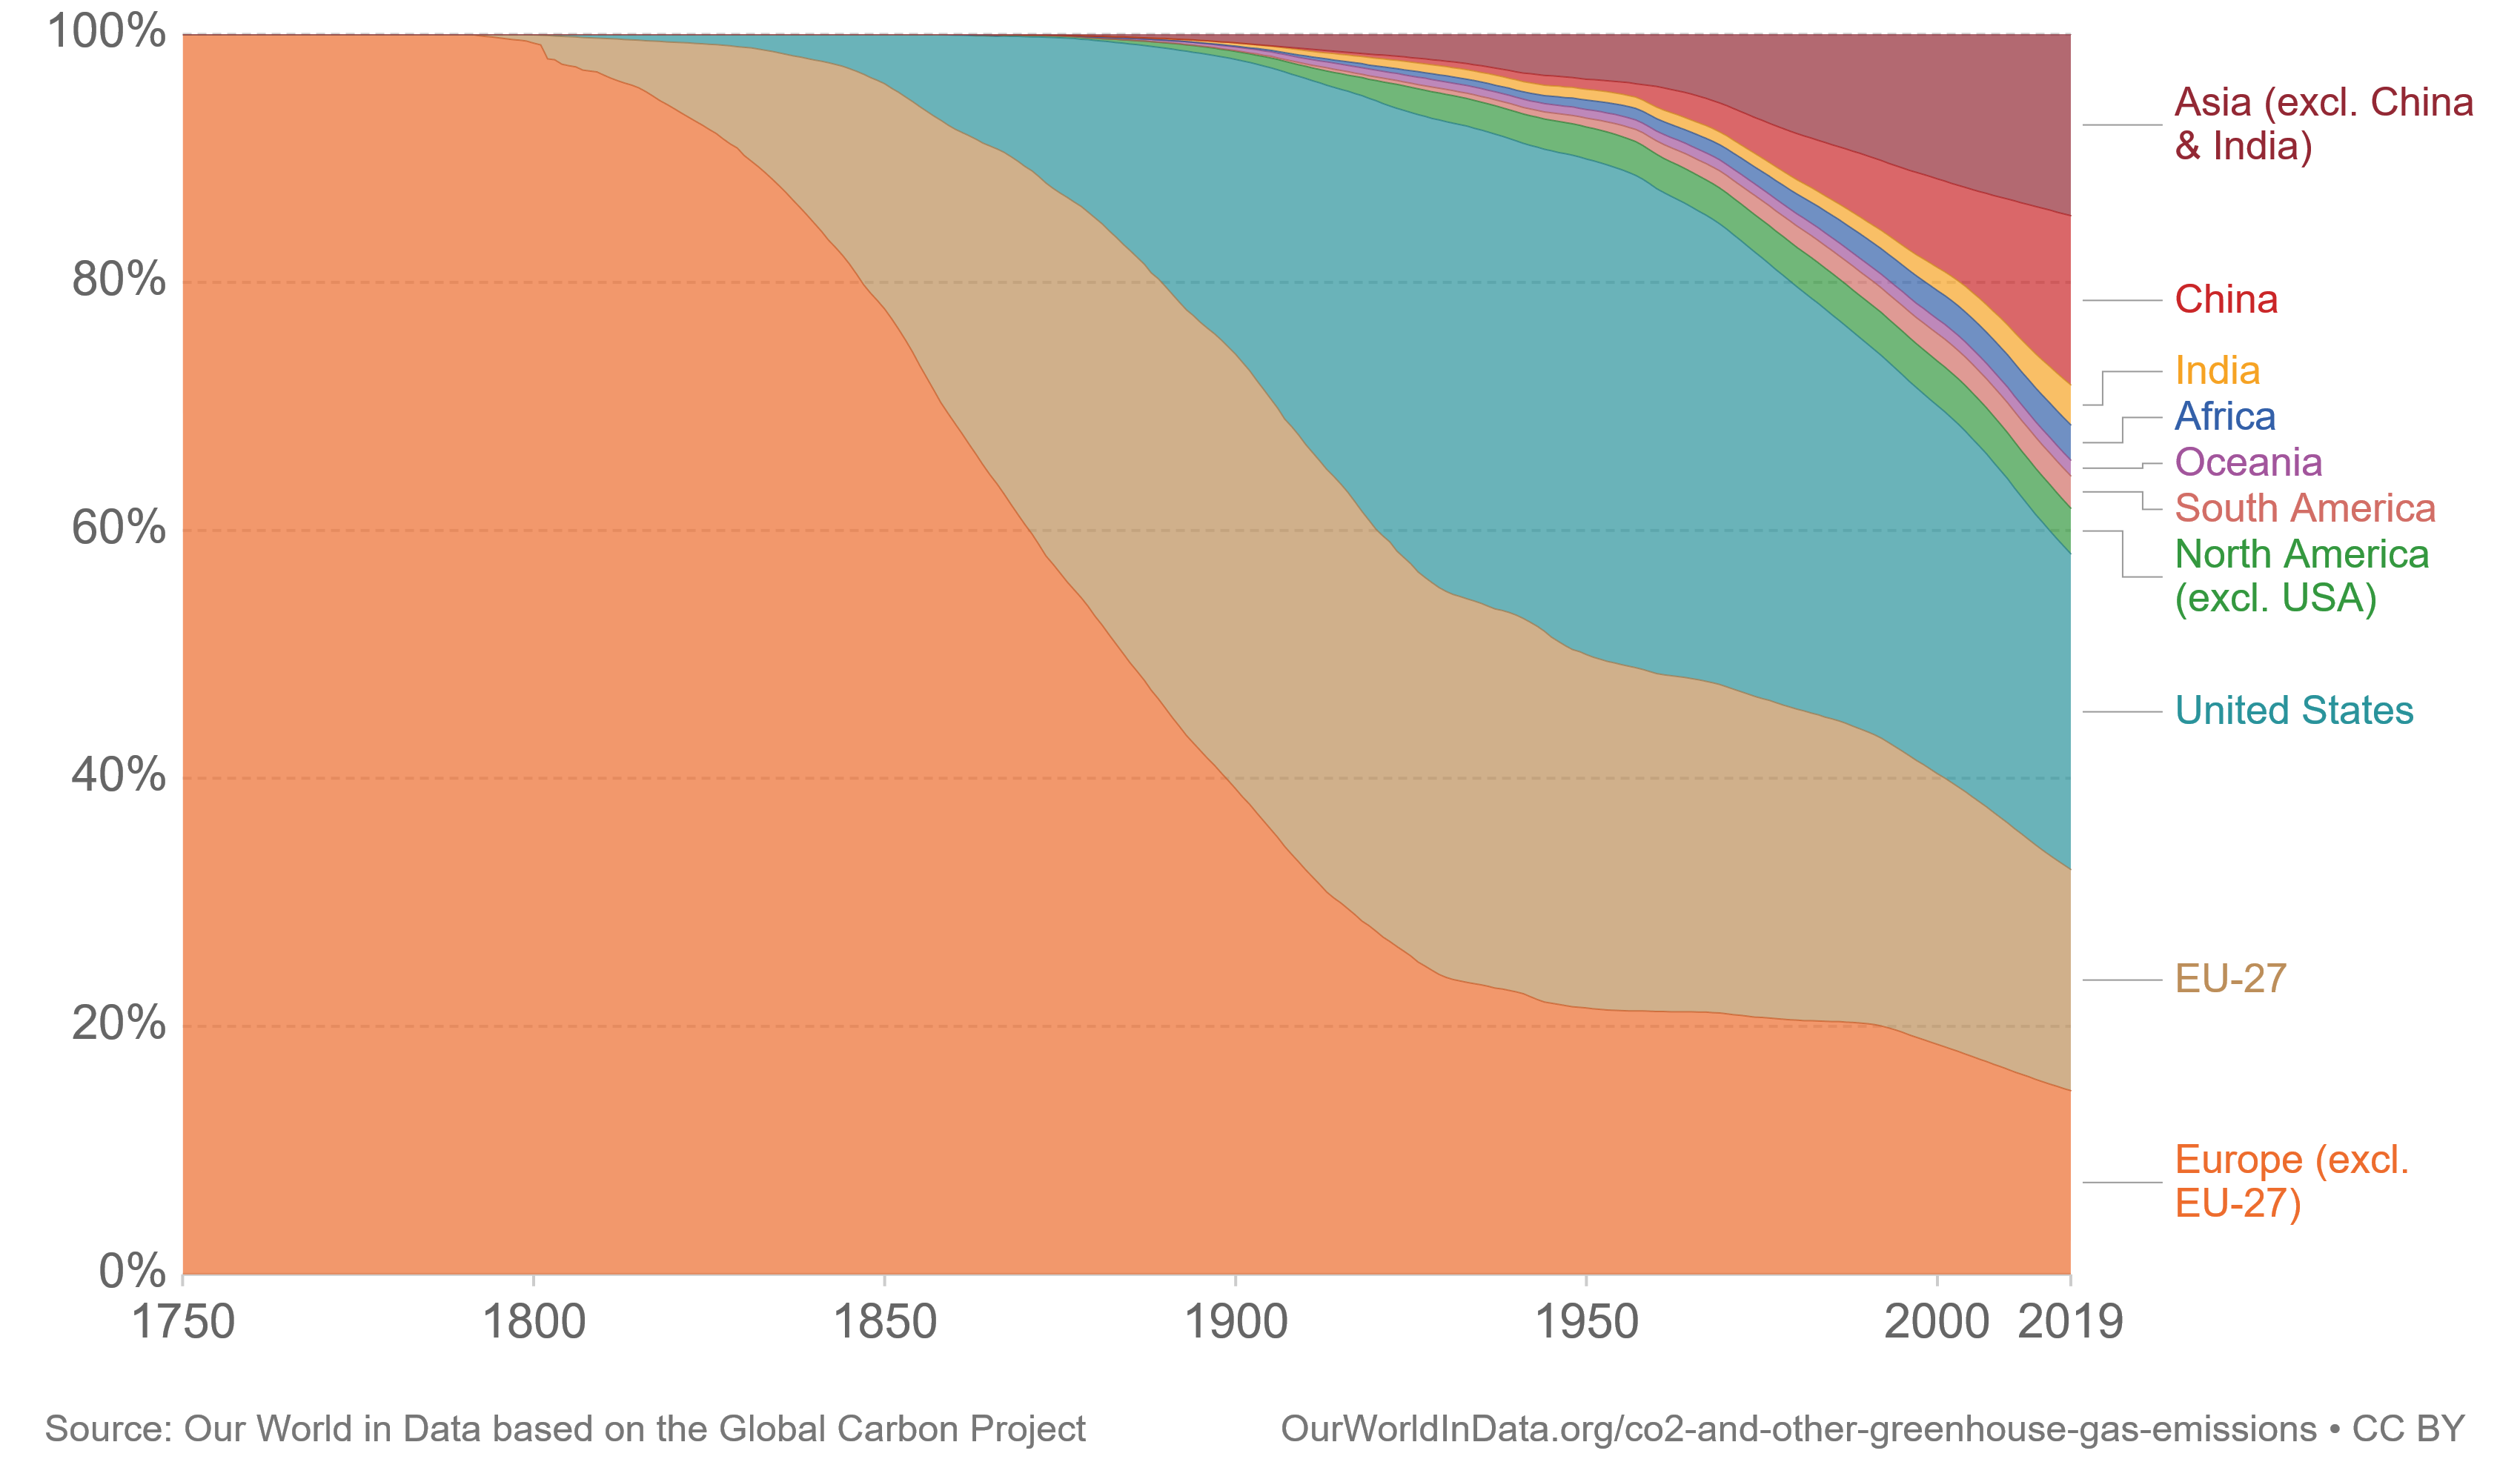
\includegraphics[width=\textwidth]{cum_emi_reg.png}
\caption{Cumulative carbon dioxide (CO\textsubscript{2}) emissions by region from the year 1750 onwards. Emissions are production-based (do not account for emissions embedded in trade). Includes CO2 emissions from fossil fuels and cement production only. Land use change is not included.}
\label{fig:hist_contb}
\end{figure}

This shift was eventually visible in the INDCs (later NDCs) --- where around 120 countries had some sort of emissions targets, around 50 countries had some type of share targets (e.g., the share of renewable in primary energy), and 15 countries had capacity targets; although many (higher or stricter) targets were conditional to international financing \citep{rogelj2017}. India and China, both significant to the future course of emissions, also announced an emission intensity and peaking year target respectively, marking a significant departure from their previous positions. 

\begin{figure}[h!]
\centering
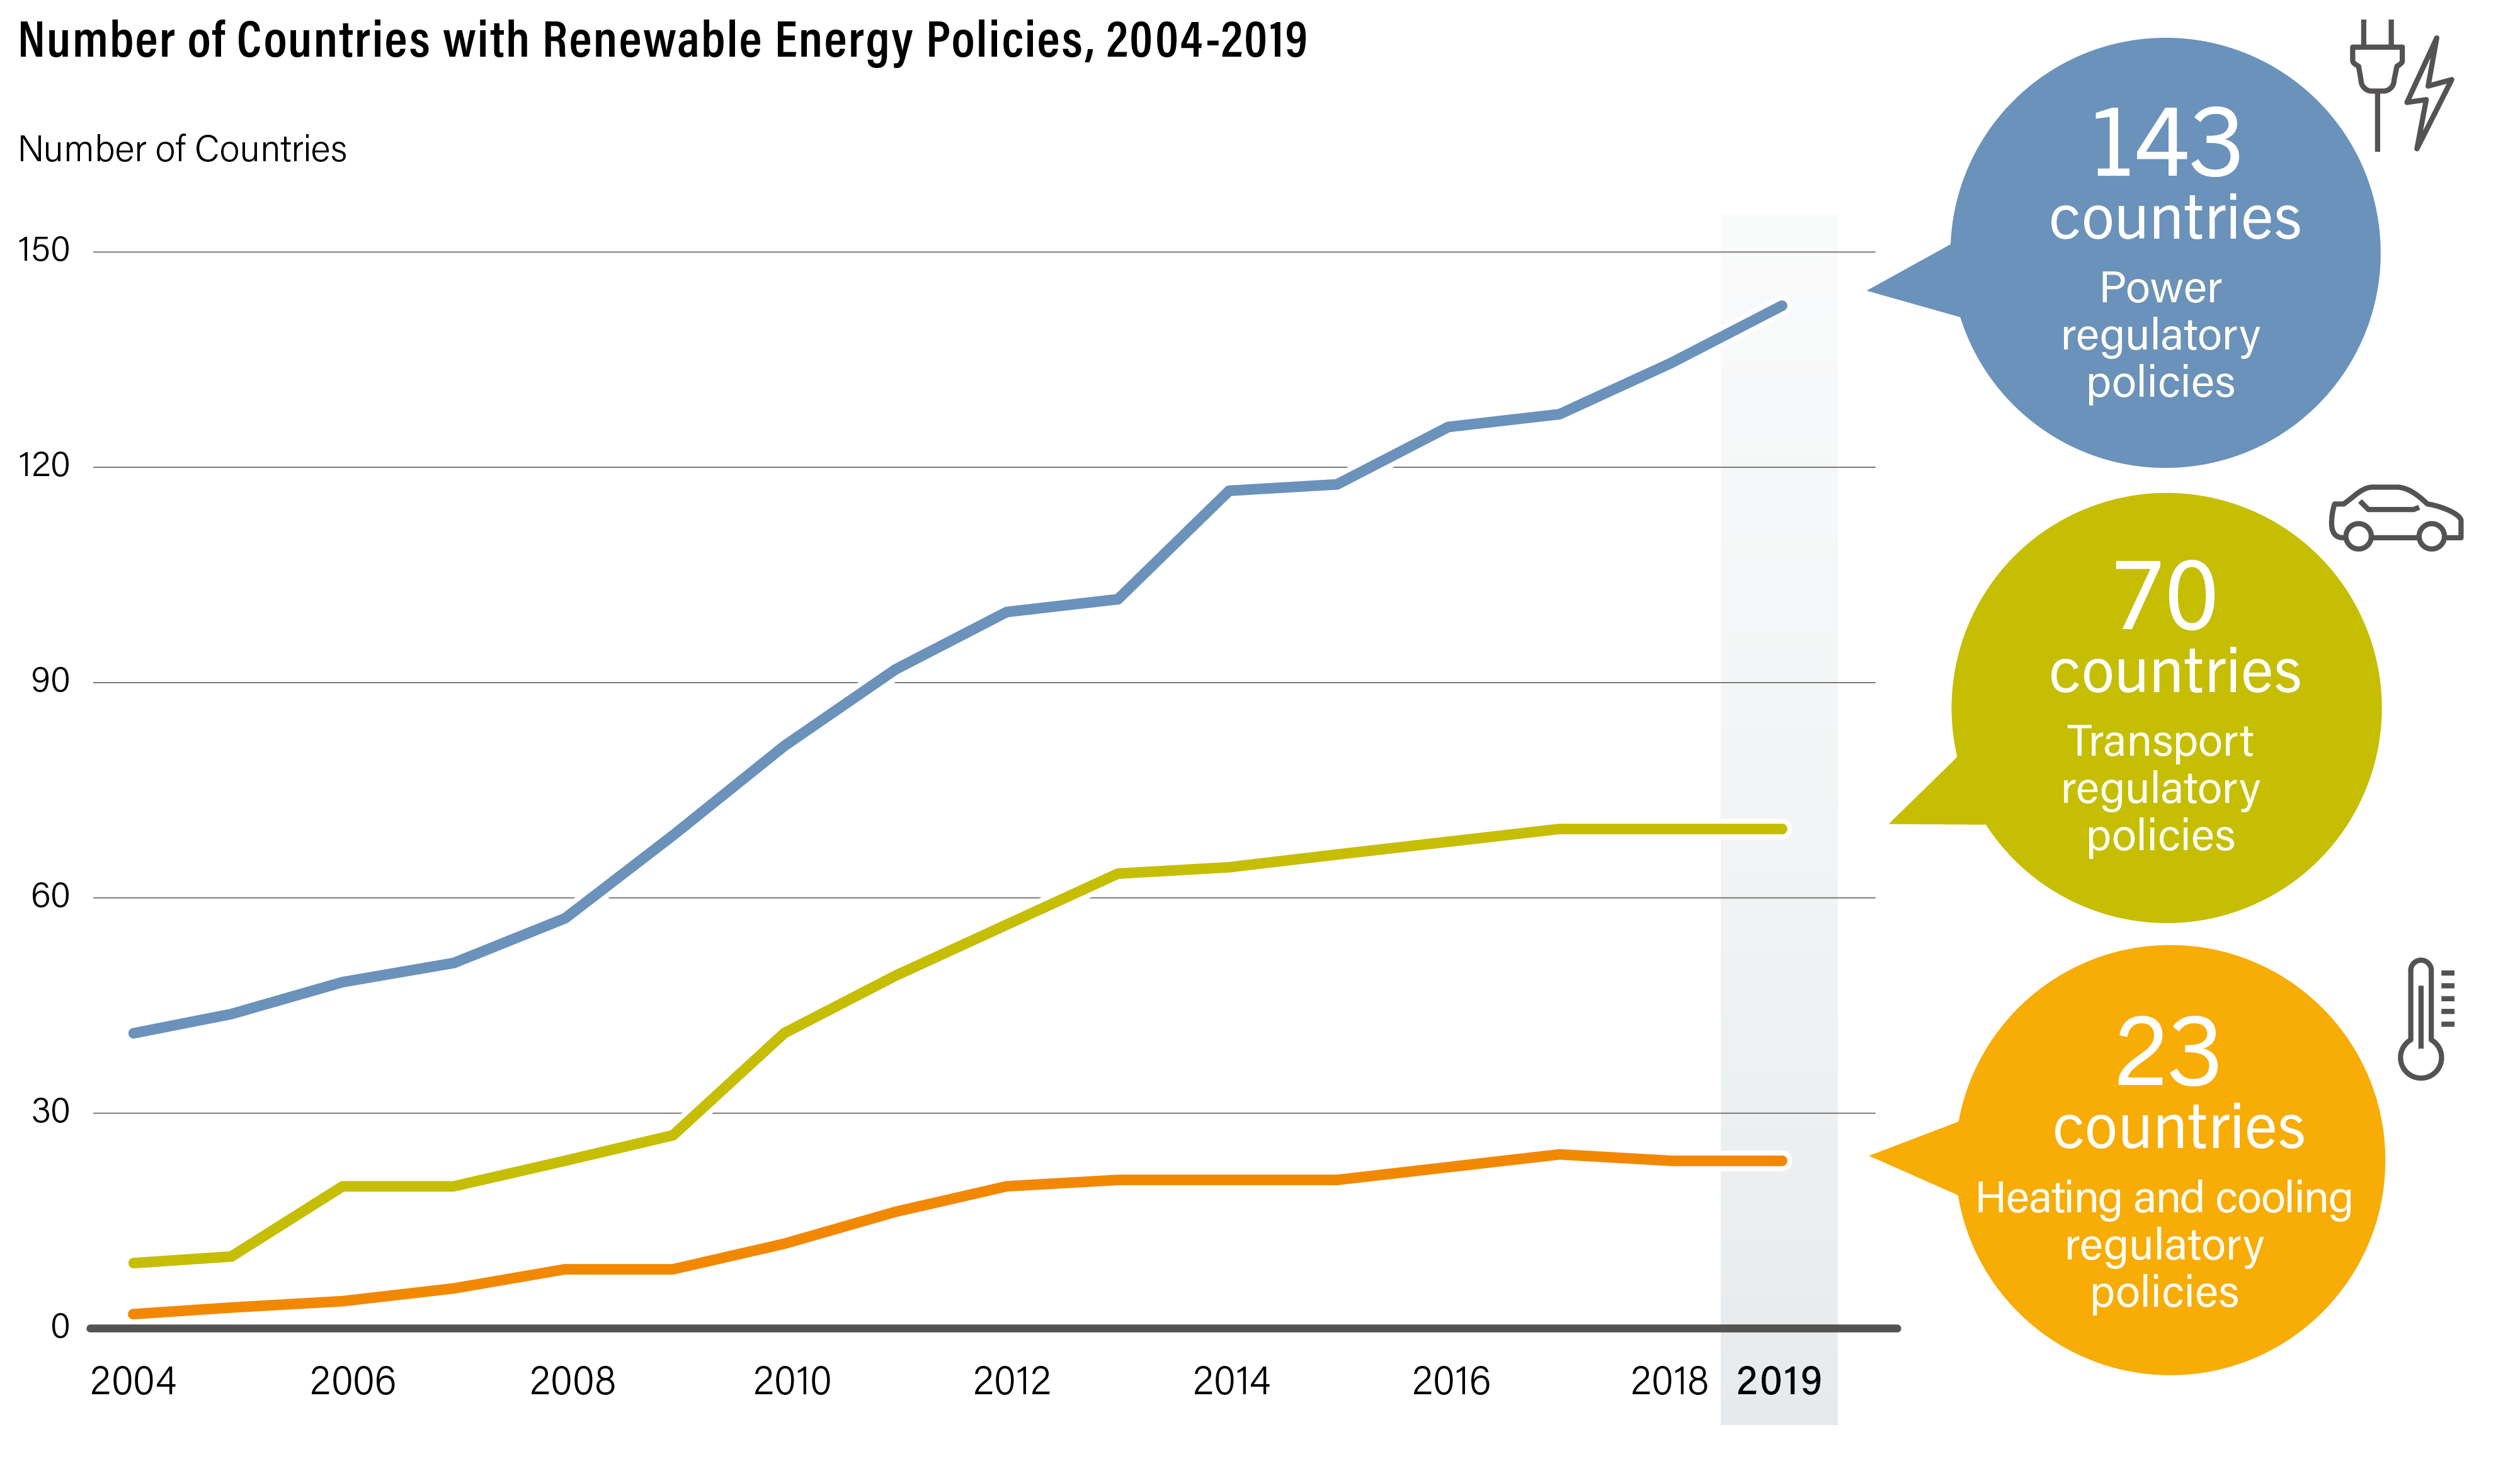
\includegraphics[width=\textwidth]{ren_policies.png}
\caption{Figure showing the number of countries with renewable energy policies from between 2004 to 2019. Power policies include feed-in tariffs (FITs), feed-in premiums, tendering, net metering and renewable portfolio standards. Transport policies include biodiesel obligations/mandates, ethanol obligations/mandates and non-blend mandates. Heating and cooling policies include solar heat obligations, technology-neutral renewable heat obligations and renewable heat FITs.  Figure and caption from \href{https://www.ren21.net/reports/global-status-report}{Global Status Report, REN21 2020}.}
\label{fig:ren21}
\end{figure}

Fast forward to 2019 and nearly all countries in the world had renewable energy support policies, although with various levels of ambition and scope; 166 countries had renewable power targets, and there were at least 56 carbon pricing initiatives in 47 countries (see \cref{fig:ren21}). As mentioned before, a part of this change came from international pressure, especially through climate negotiations. However, several other factors have provided further impetus to decarbonisation:
\begin{enumerate}
\item Driven by a drastic drop in prices of photovoltaic modules and wind turbines and RE support policies, new RE-based power generation became more cost-effective than new coal-fired plants in nearly all countries \citep{ren212020}. In India and China, it became even cheaper to build new RE than operate some existing coal power plants \citep{runyon2021}.
\item There was an increasing understanding that many of the objectives of developing countries (e.g., energy access, energy security, improving human health) could also be achieved (or at least be complemented) through enhanced climate action (co-benefits) \citep{dubash2013politics}: many developing countries have abundant solar/wind energy but limited or no fossil fuels, therefore RE could provide energy security and even reduce fossil fuel import bills over the long-term \citep{iea2021}; energy access in rural areas could be better achieved through decentralised RE than fossil-fuel-based systems \citep{arent2017}; air pollution benefits from a coal phase-out alone could be sufficient to warrant action, even without considering climate impacts \citep{rauner2020}.
\item Lastly, through continued research on climate impacts, including the observed increase in impacts in most parts of the world \citep{williams2019}, it became increasingly clear that climate impacts could significantly push back development gains \citep{dubash2019}, with developing countries being much more vulnerable and thus, mitigation at home and strong climate action internationally were important for national interest \citep{thaker2014shifting}. 
\end{enumerate}

Armed with strong reasons to decarbonise, the starting point for most low-income countries was the power sector, as also illustrated in \cref{fig:ren21}, which shows the increasing adoption of power regulatory policies. Moreover, a decarbonised power sector was also an essential foundation for future decarbonisation of other sectors, e.g., transport and heating. The next section describes the pathways to power sector decarbonisation along with its various challenges.

\subsection{Power sector decarbonisation}
The power sector, alternatively called the electric power sector, ``consists of electricity only and combined heat and power (CHP) plants whose primary business is to sell electricity, or electricity and heat, to the public'' \citep{eia}. In the year 2018, the sector contributed to \textasciitilde \SI{30}{\percent} of all greenhouse gases (GHGs) emitted in the world \citep{climatewatch}. In the last ten years, emissions from the sector have increased by \textasciitilde \SI{10}{\percent}. The decreases in emissions from the EU and the US (mainly through the switch from coal to cheaper gas) more than offset by increasing coal-powered generation in China and India (see \cref{fig:hist_power_emi}).

There are indications that emissions in the sector could have already peaked in 2018, especially if the growth of low-carbon energy outpaces future demand growth \citep{bertramCOVID192021,lolla}. As mentioned before, RE (especially solar energy) is now cheaper than new coal power in both China and India, where a significant share of future demand is estimated.

\begin{figure}[h!]
\centering
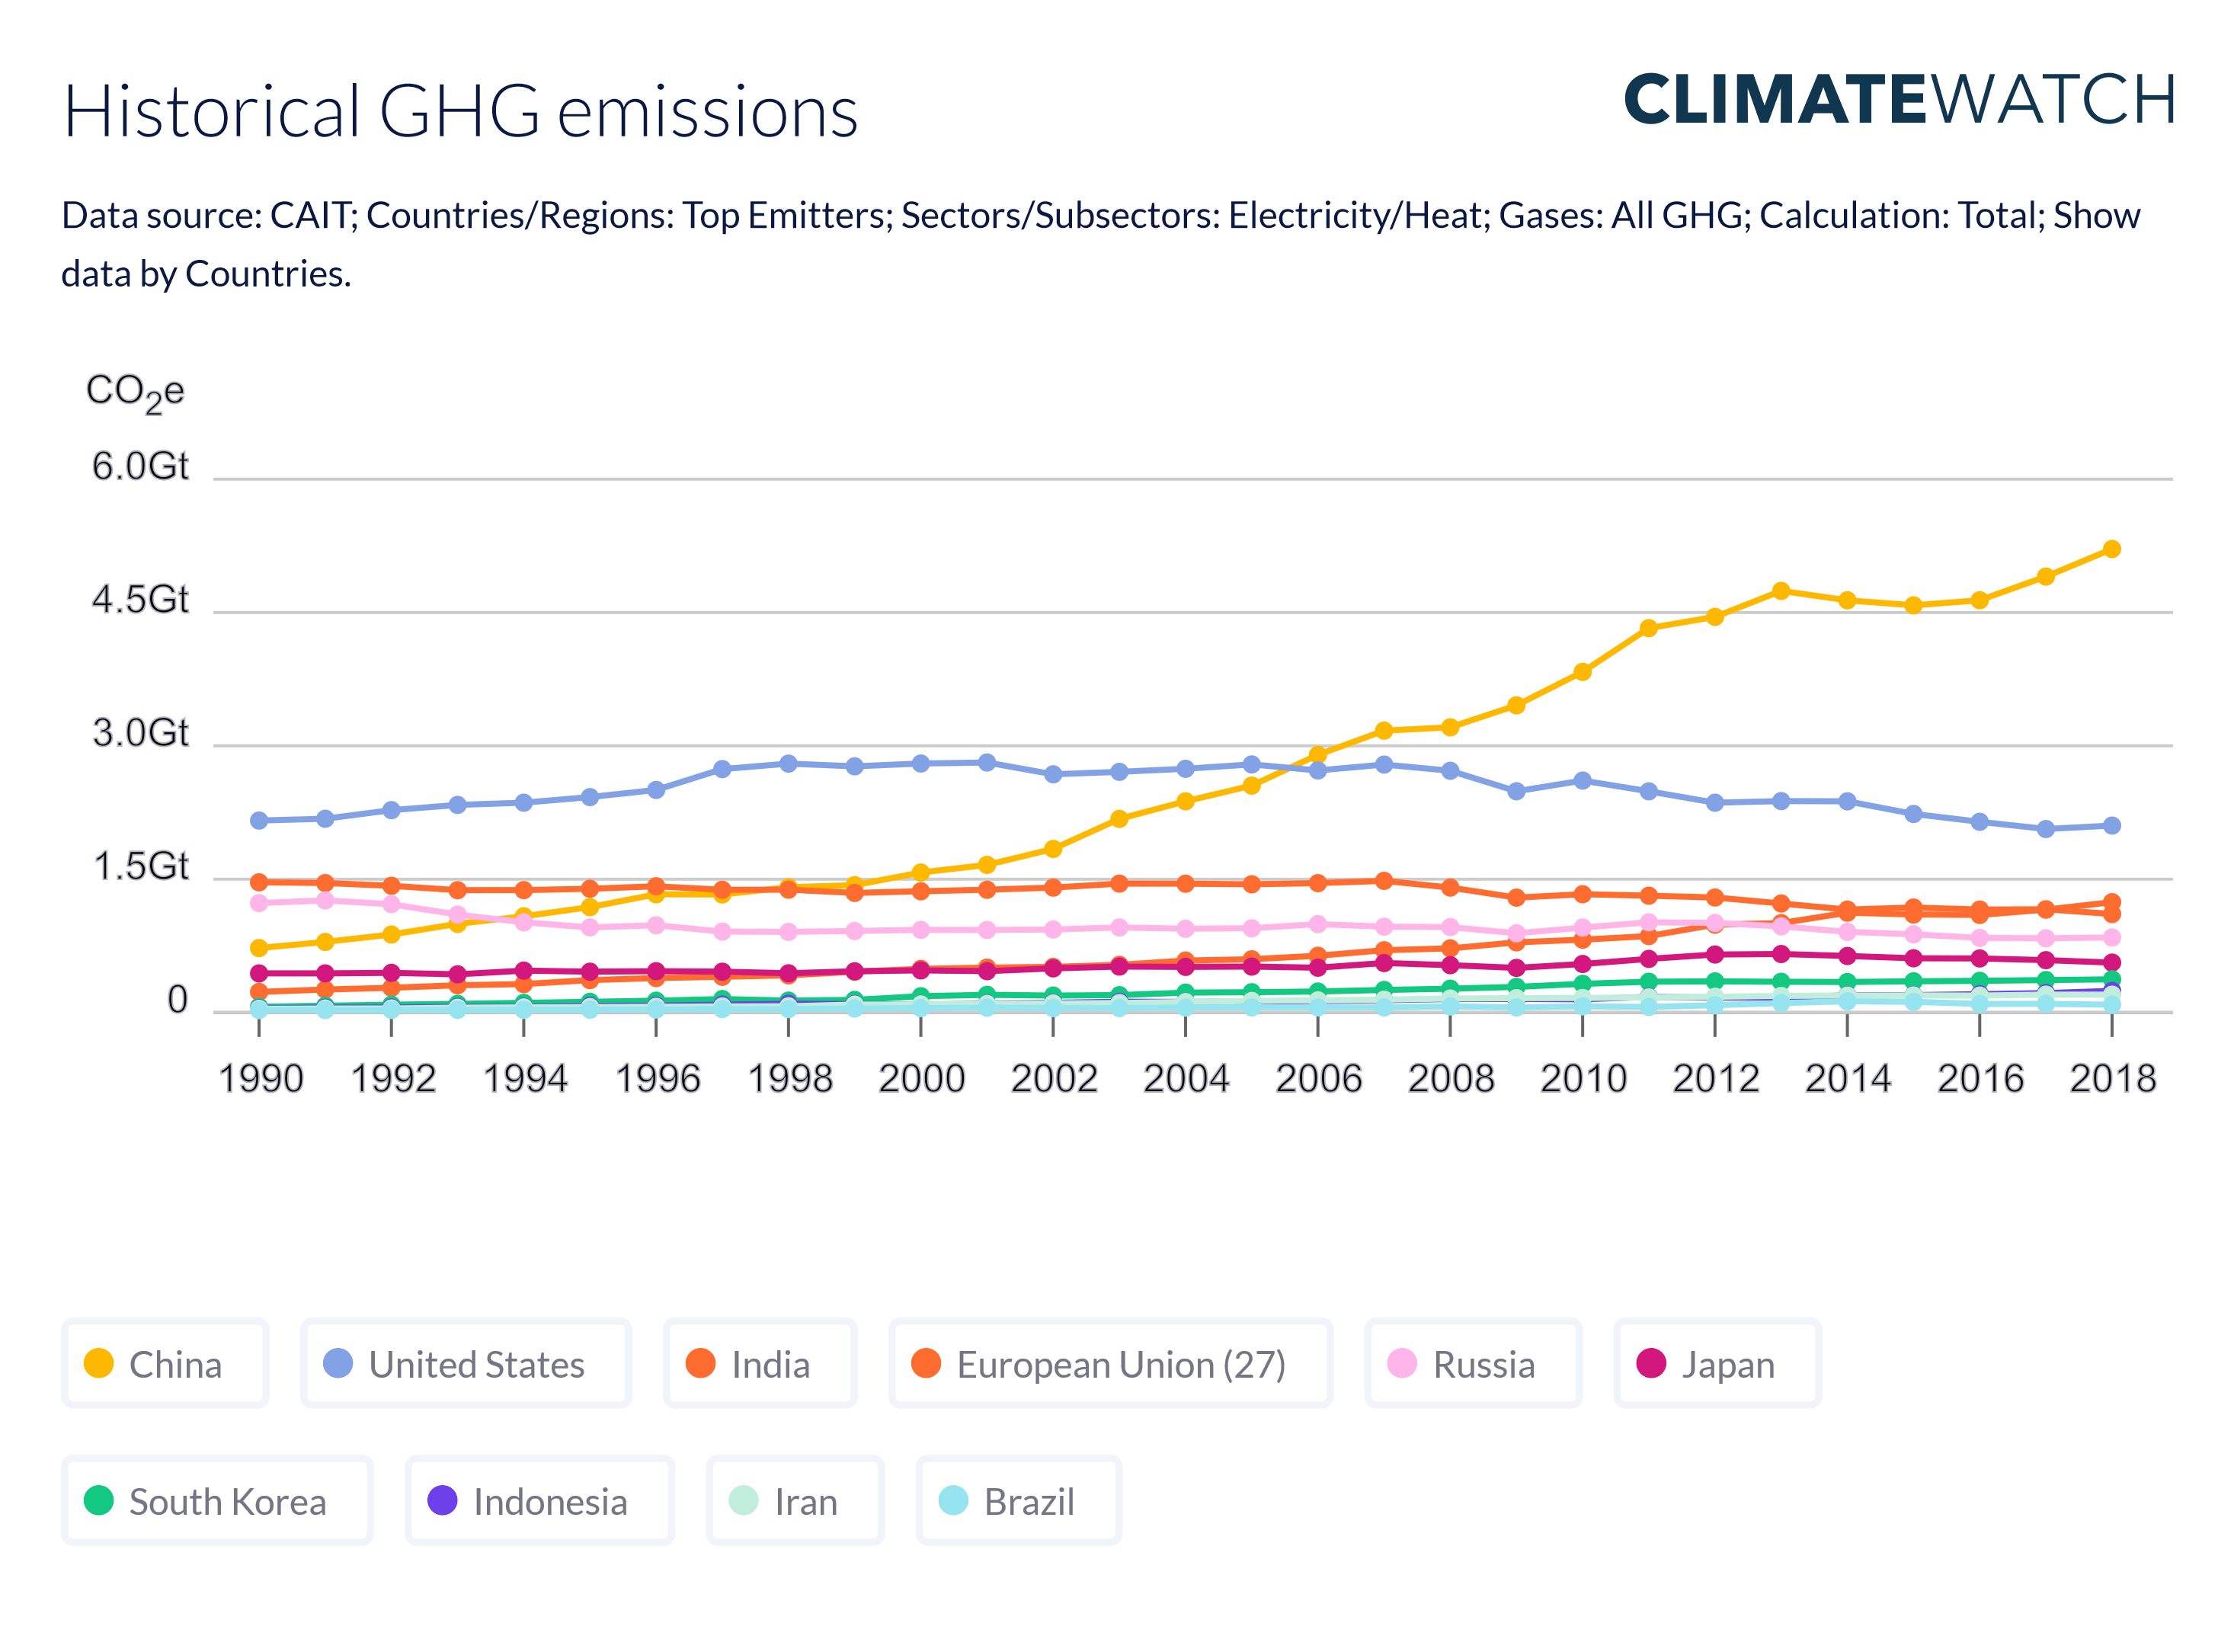
\includegraphics[width=\textwidth]{historical-ghg-emissions.png}
\caption{Historical emissions from the power sector, in Gigatonne (Gt) CO2 equivalent, from 1990 to 2018. Figure from \url{climatewatchdata.org}}
\label{fig:hist_power_emi}
\end{figure}

\subsection{Political economy of decarbonisation and the role of just transition}\label{subsec:near_term}

Mitigation pathways have traditionally been relied on techno-economics, focusing on including a wide array of technologies which can be used to decarbonise the different sectors :electricity generation, industry, transportation, and buildings.  In the process they have answered questions on `how much to invest, in what, and by what time?'. However, as power-sector decarbonisation became increasingly mainstream and essential in policy-making, real-world discussions have also become more political and nuanced, with a focus on the near-term. In turn, this has led to calls to include dimensions of (political) feasibility in mitigation pathways \citep{anderson2019} and explore near-term policies which can effectively reduce emissions and provide development gains and/or pass through political or economic hurdles.

Several studies have eventually explored these connections. \citet{pahle2018a,meckling2015winning,green2018cutting},  e.g., argue that although policies favouring low-carbon such as feed-in tariffs \footnote{``A feed-in tariff is a policy tool designed to promote investment in renewable energy sources. This usually means promising small-scale producers of the energy — such as solar or wind energy — an above-market price for what they deliver to the grid'' \citep{willkenton2021}}, R \& D subsidies, etc.\ (also called supportive supply-side policies) or fossil fuel ban/moratorium etc. (also called restrictive supply-side policies) are considered suboptimal as policy options (compared to carbon-pricing), they have numerous economic and political advantages - e.g., they can create (counter) constituencies to fossil fuels in the renewable energy industry and produce their lobbying efforts. \citet{rauner2020,west2013} show that linking air pollution to mitigation also has immense potential to achieve wide agreement and ease feasibility. \Citet{iyer2015} show that the high upfront capital costs associated with solar and wind generation, and the higher perceived risk of investment in developing countries (leading to higher financing costs), implies that financial constraints could prevent low-carbon investment in these countries, possibly locking them into carbon technologies. Lastly, \citet{mccauley2018,healy2017} argue that the energy transition will fail to gather pace unless losers of the transition (be it businesses, states, or unions), especially those who are poor or spend significant income on acquiring energy, are not adequately compensated (e.g., through recycling of carbon tax revenue) or not involved in the decision-making process. These will be elaborated on in the subsequent sections.

The idea behind \textit{just transition} is that people, communities, and regions who stand to lose the most from an energy transition undergo an inclusive and planned shift to alternate means of income and sustenance, or get adequate compensation. To a lesser extent, it also implies that the benefits from a transition, in the form of additional jobs created in the supply chain, better air (through cleaner power plants), or cheaper power are not concentrated in certain regions. The worst instance would be e.g., that affected regions and people are not compensated in any way and renewable-related infrastructure is constructed and developed in far-off regions, ultimately forcing the people to emigrate to look for a better life or if they are too old to acquire new skills or jobs, remain unemployed.

The concept of just transition first emerged from trade unions in the 1970s in the US against the loss of jobs from environmental policies \citep{morena2018}. They acknowledged that although some industries were leading to local environmental and health problems, simply shutting them down was not a reasonable solution, and instead, public policies should focus on addressing environmental problems, simultaneously securing decent jobs and livelihood for the affected workers \citep{morena2018}. The just transition movement gained widespread agreement and popularity in the US, but it was only in the early 2000s, through other trade unions in the Global North and supported by powerful groups like the International Trade Union Confederation (ITUC), that its ideas diffused into mainstream climate negotiations \citep{morena2018}. The term was repeatedly used in various COPs, eventually leading to the adoption of the \textit{Solidarity and Just Transition Silesia Declaration} in COP 24 in Katowice, Poland (2018) by 52 countries, with the aim of main-streaming its message in global climate policy \citep{cop24}. In the last few years, several countries, especially those belonging to the Powering Past Coal Alliance (PPCA) have put forward proposals or policies to promote just transition\footnote{Examples include the `Task Force on Just Transition for Canadian Coal Power Workers and Communities in Canada' \citep{canada2018}, in the EU through the 17.5 billion \texteuro  `Just Transition Fund' \citep{eu_just}, in Germany through the `Coal Commission - A Roadmap for a Just Transition from Coal to Renewables' \citep{litz2019}.}. 

A number of recent studies have tried to quantify the elements of a just transition, although often limiting their scope to `workers in coal-regions' and seeking their alternative re-employment or retraining opportunities in low-carbon industries. \Citet{kapetaki2020}, focusing on the EU, identify the jobs and regions, set to lose most from a decline in coal mining and provide estimates of how clean energy deployment, including energy-efficiency measures could (positively) impact job creation and regional economic development. For the latter, they also look at what industries in the value-chain (e.g., nacelle manufacture for wind turbines, RE developers, battery production) already exist and thus be more conducive to particular transition solutions. \citet{pai2020} look at the locations of coal mines in four countries (United States, China, India, and Australia) and analyse if areas around these regions are conducive to solar and wind installations. They then estimate how much RE capacity would need to be installed to re-employ everyone in the coal mining sector. They focus only on O \& M jobs in RE, due to their long-term job security, similar to coal mining jobs. \citet{briggs2020}, focusing on Australia, look at the transition from a more occupational viewpoint, i.e., which jobs in the coal sector overlap with RE jobs, and what people could be retrained easily to the latter. \citet{dominish2019} compare (globally) types of occupations in the energy sector across in different mitigation scenarios and find that ``jobs created in wind and solar PV alone are enough to replace the jobs lost in the fossil fuel industry across all occupation types''. Lastly, \citet{bhushan2020} attempt to ascertain the dependence of coal mining on the communities living around it \footnote{they do this for the district of Ramgarh using primary surveys.} and use the knowledge to create a just transition framework for India. Unlike other studies focusing particularly on renewable energy, they look into greater depth at alternate livelihood opportunities and economic diversification; although only qualitatively.

\section{Conceptual framework --- barriers to power sector decarbonisation}\label{sec:framework}
The barriers to power sector decarbonisation can be broadly grouped into three categories: \textit{techno-economics}, \textit{governance and institutions}, and \textit{socio-economic and political barriers} (\Cref{fig:graphical_outline_prev}). The framing of these barriers is similar to that of carbon lock-ins first elicited by \citet{unruh2000} (also used to understand barriers to mitigation) and eventually adapted and expanded by \citet{seto2016}. However, the present classification is purposely broader to include elements not fully considered in the carbon lock-in approach, e.g., energy justice and financial considerations (access to capital). The classification is useful to understand that each classifier has actors who try to fulfil their own interests (or have their limitations) and systems that have their characteristics --- e.g., the election cycle, the long lifespan of carbon infrastructure, etc. The three classifiers are briefly discussed below:

\begin{figure}[hbtp]
\centering
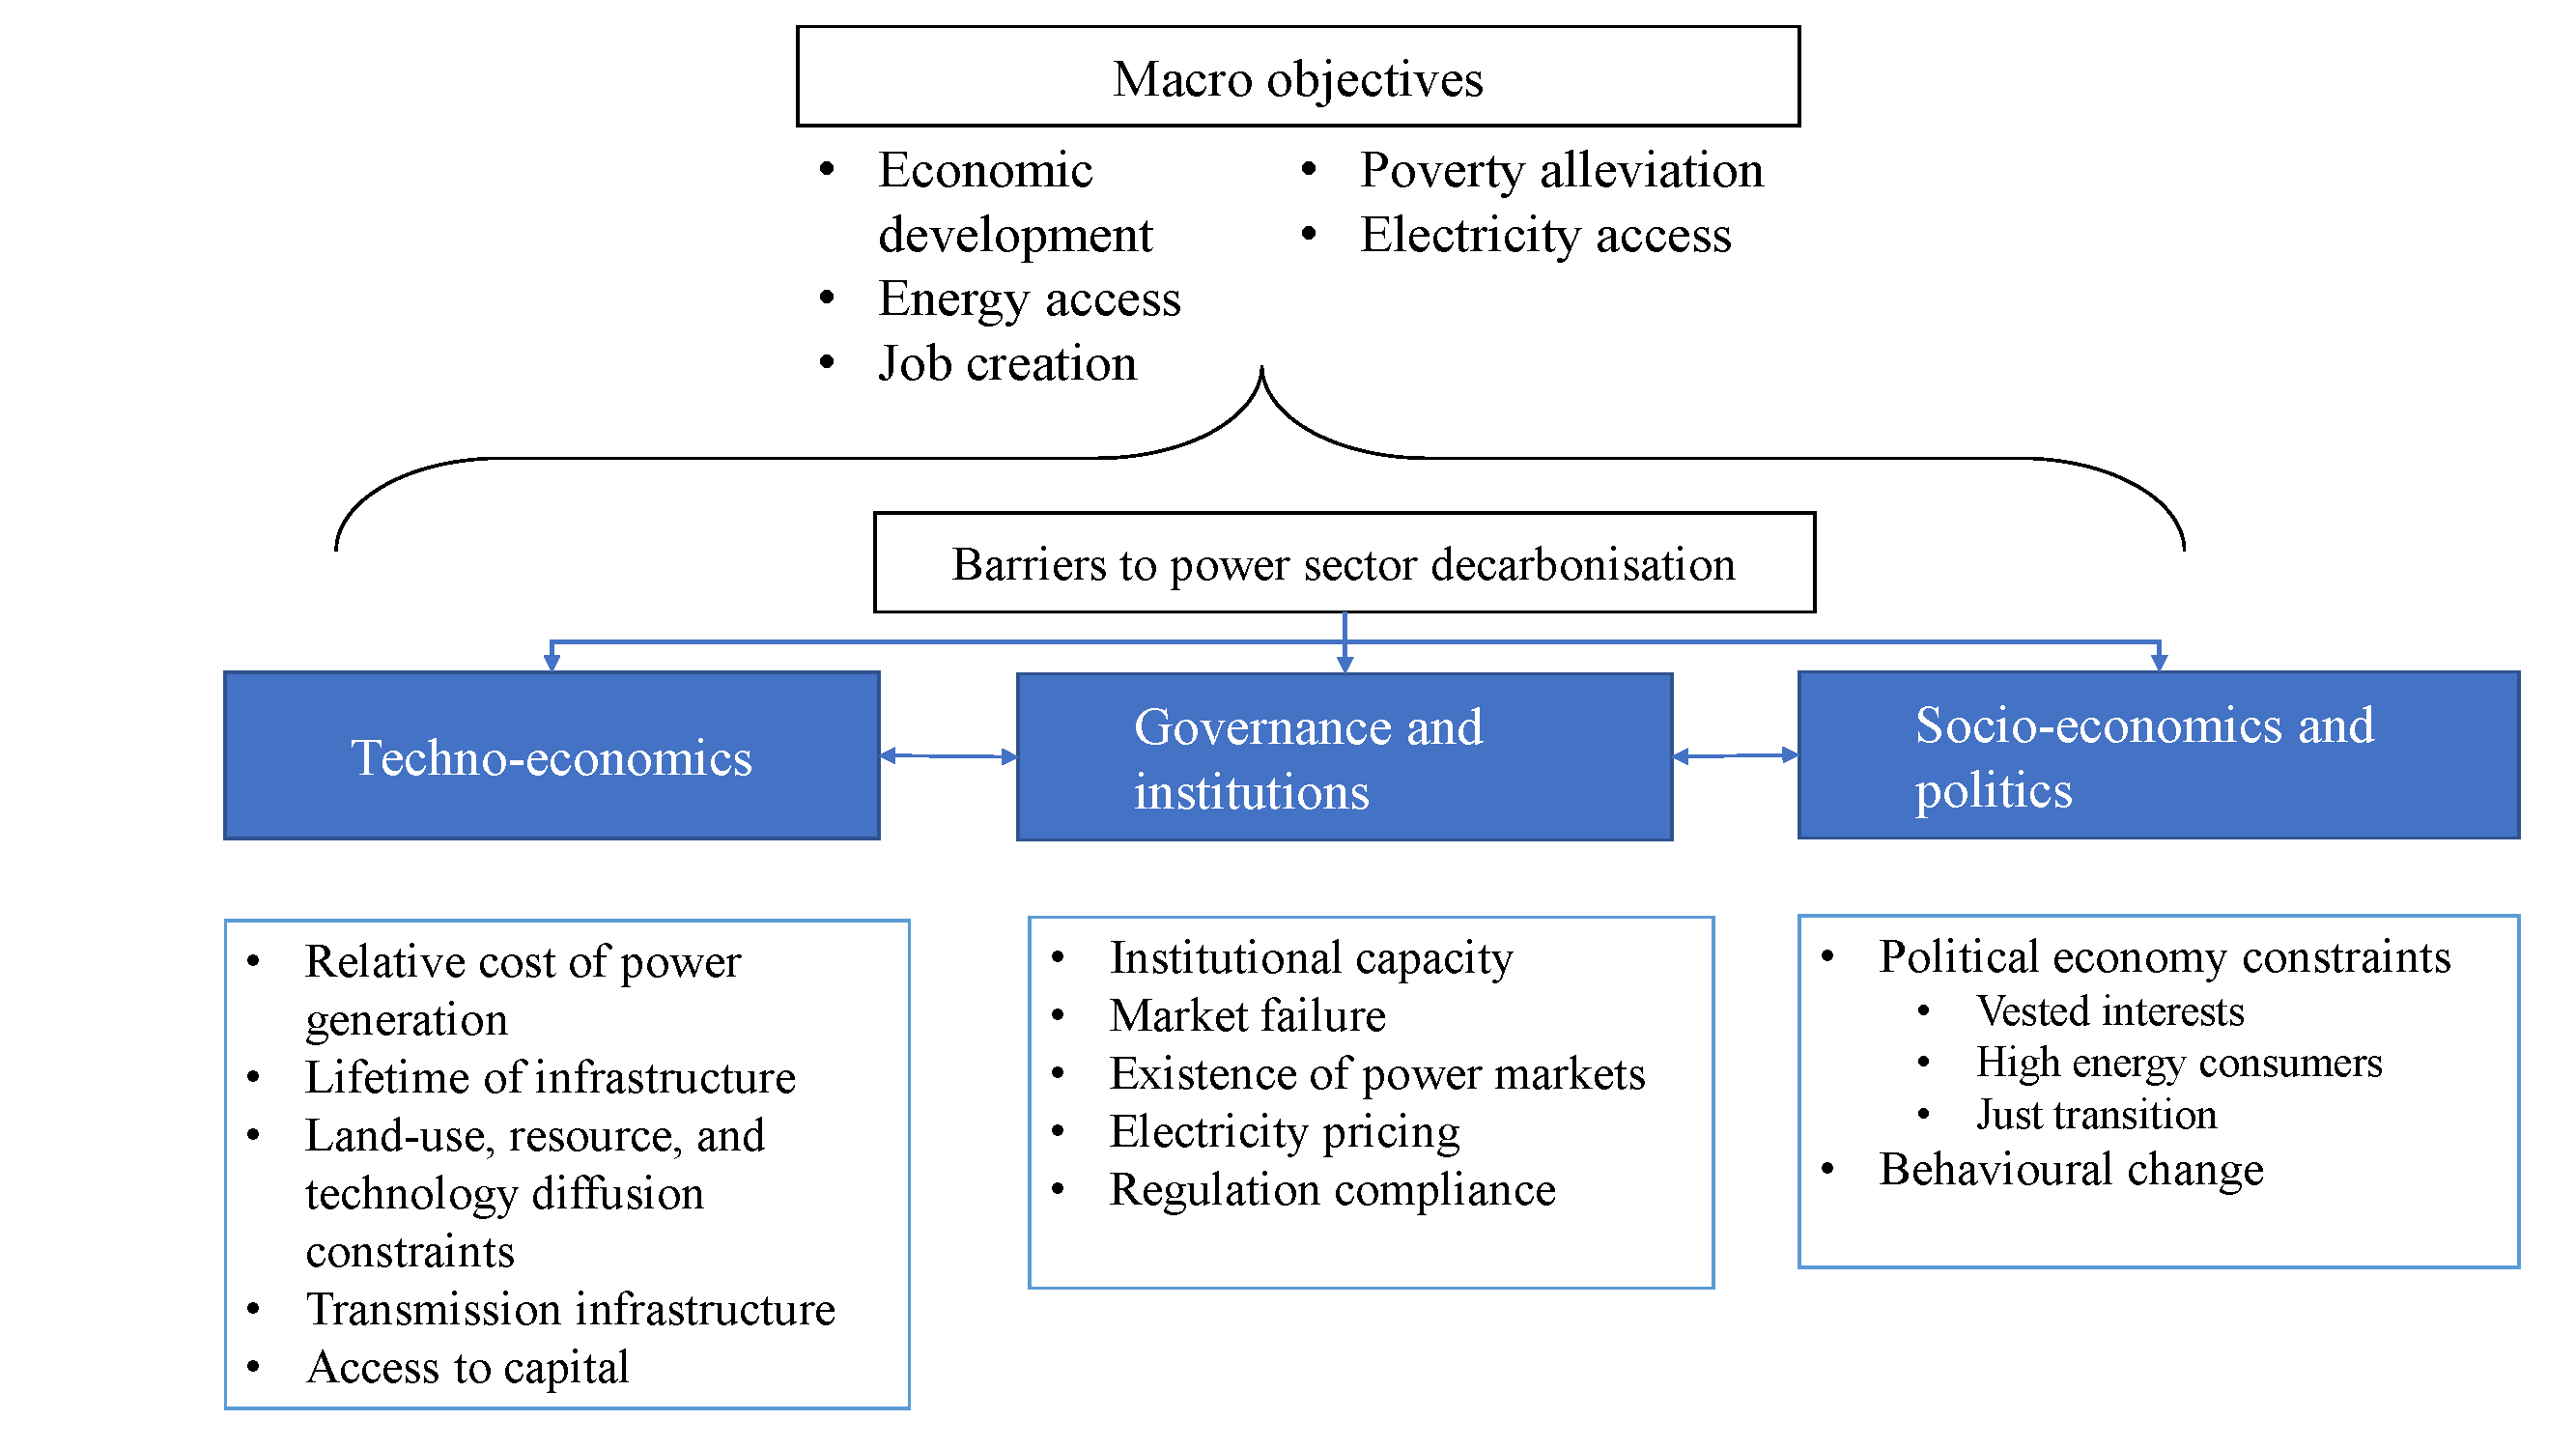
\includegraphics[width=\textwidth]{graphical_outline_prev.png}
\caption{Conceptual framework of the thesis classifying the barriers to power sector decarbonisation}
\label{fig:graphical_outline_prev}
\end{figure}

\begin{enumerate}
\item \textbf{Techno-economics}. The techno-economic barriers refer to the relative costs of different power generation technologies, specifically the costs associated with developing a low-carbon power infrastructure compared to a more passive fossil-based power system. Additional constraints like land can become important in regions of high population density or limited suitable sites. Moreover, high upfront capital requirements (difficulty in accessing finance) can prevent the growth of solar and wind, even if it is competitive to fossils. Lastly, the long lifetime of power infrastructure creates path-dependency preventing optimal outcomes in the future (carbon lock-ins).

\item \textbf{Governance and institutions} refer to how the power system is governed including the structure of its institutions along the whole life-cycle --- starting from generation to transmission-and-distribution (T \& D) and eventually consumption. Barriers here include the short time horizons of politicians which make them risk-averse to potentially disruptive technologies or in other words, continue following the status quo. They could also be in form of limited institutional capacity, e.g., although climate action and sustainable development cut across traditional sectors, work between them may not be aligned; it could also mean limited know-how on how to connect traditional objectives with mitigation objectives \citep{dubash2019}.

\item \textbf{Socio-economic and politics} concerns mainly with political economy constraints and behavioural change. The former refers to consumers, citizens, and corporations who will be negatively affected by an increase in costs of fossil fuels and will therefore try to oppose change or lobby for weaker change \citep{jenkins2014}. On the other spectrum, it might impact the access to food and energy of the world's poor \citep{fujimori2019}. At a larger scale, decarbonisation has been opposed by nations and nation-states which receive significant revenue through fossil fuels. Decarbonisation policies must therefore address these constraints through additional policy measures. 
Behavioural change refers to the (individual) patterns and habits of food, mobility, and housing requirement expressed partially through metrics like ecological footprint and carbon footprint. Constraints resulting from resistance to changing habits are less important in power sector decarbonisation and more relevant for land-use emissions \citep{vandeven2018}.
\end{enumerate}

\section{Research objectives}\label{sec:objectives}
For the major part, this thesis \textbf{focuses on the barriers to power sector decarbonisation in India}. This is because: Firstly, although India is currently the world's third-largest emitter, it's share of historic emissions has been low and its per capita electricity and energy consumption are still well-below the world average. Millions of people still don't have access to reliable electricity and clean energy. Secondly and consequently, this means that India is projected to have the fastest growing electricity market in the world over the next decade \citep{buckley2015}; according to India's nationally determined contribution (NDC), ``half of the India of 2030 is yet to be built''. Thus, how it meets its future energy demand, particularly electricity, has important implications for itself and the rest of the world. Lastly, India has one of the largest reserves of coal and is currently the second largest coal consumer in the world after China. Coal and coal-based electricity plays an important role in national and regional politics. Thus, any alternatives to coal need to have strong economic arguments and need to be able to deliver increasing power generation both cheaply and reliably.

The research objectives of the thesis were identified based on the underlying conceptual approach described in \Cref{sec:framework} and assessing the gaps in existing literature. These gaps could be thematic e.g., focusing on political factors that influence the pace of decarbonisation instead of the usual techno-economics but also methodological, e.g., comparing results between different types of models. This approach led us to three principal objectives, enumerated below:

\begin{enumerate}

\item How could near-term policies in India impact longer term decarbonisation efforts required to achieve Paris Agreement targets? What set of decarbonisation options does India have in the near- and long-term? 

\item How do different decarbonisation scenarios change the number and structure of jobs globally and within major countries in the energy sector and what impact does it have on the success of decarbonisation policies?

\item How do current energy policies and strengthening of RE targets in India and its different states impact the distribution of energy assets and energy jobs across the country and how could it affect the pace of decarbonisation viz. the concept of just transition?

\end{enumerate}


\section{Methodology}
The objectives in \Cref{sec:objectives} are investigated using different methodological tools which are summarised in \Cref{tab:meth_tab}. Special focus is given on the near-term and on bridging model results with bottom-up developments in the energy sector. The key concepts and indicators of each study are also mentioned in \Cref{tab:meth_tab} and explained in detail in the subsequent subsections.


\begin{table}
    \centering
    \begin{tabularx}{\textwidth}{|p{1cm}|p{1.5cm}|p{1.6cm}|X|X|}
    \hline
         & \textbf{Spatial focus} & \textbf{Temporal focus} & \textbf{Methodological tools used} & \textbf{Key concepts and indicators}  \\ \hline
        Ch. \ref{ch:ERLPaper} & India & 2030 and 2050 & IAMs, national energy models, model intercomparison, bottom-up data on policies and planned capacities, scenario development & IAMs (\Cref{subsec:iams}), model intercomparison ( \Cref{subsec:model_inter,subsec:glonat}), stranded assets and committed emissions (\Cref{subsec:comm_stranded}) \\ \hline
        Ch. \ref{ch:EnPolPaper} & Global and large regions & 2030 and 2050 & Employment-factor approach, IAMs, scenario development & Estimating energy employment, including employment-factor approach (\Cref{sec:employment})\\ \hline
        Ch. \ref{ch:ERLPaper2} & sub-regions in India & 2030 & Employment-factor approach; IAMs; scenario development; bottom-up data on operating, under-construction, and planned energy infrastructure; just transition & See cell above and discussion in \cref{subsec:near_term} \\ \hline
    \end{tabularx}
    \caption{Key methodological tools, concepts, and indicators employed in the thesis}
    \label{tab:meth_tab}
\end{table}
\subsection{Integrated Assessment Models}\label{subsec:iams}
Integrated Assessment Models (IAMs) are numeric models representing features and interactions of natural and human systems, thereby combining knowledge spread across various disciplines \citep{weyant1995integrated,rogelj2018}. The integration allows understanding and insights not usually available through disciplinary research.  The main objective of IAMs is to inform policy and decision-making e.g., by analysing policy impacts towards a given goal, analysing benefits and trade-offs of policies across different sectors, and setting research priorities \citep{weyant2017}. According to \citep{wilson2021}, these models

\begin{enumerate}
\item represent explicitly the drivers and processes of change in global energy and landuse systems linked to the broader economy, often with a high degree of technological resolution in the energy supply.
\item capture both biophysical and socio-economic processes including human preferences, but do not generally include future impacts or damages of climate change on these processes
\item project cost-effective `optimal' mitigation pathways under what-if assumptions or subject to pre-defined outcomes such as limiting global warming to \SI{2}{\degreeCelsius} \citep{sathaye2013methods}
\end{enumerate}

\subsubsection{Differences in process-based models}
In general, IAMs are grouped into broad categories. The first, called benefit-cost models includes the more stylised IAMs like DICE, RICE, FUND, etc. which have simplified representations of energy and land-use systems and are, as the name suggests, often used for cost-benefit analyses. The second class, called process-based or detailed-process models, include a  detailed representation of regions, sectors, and technologies and can thus a provide wide variety of scenarios \citep{weyant2017}. This thesis exclusively focuses on the latter. 

Process-based models further differ from each other on numerous aspects, some of which are captured by \citet{krey2014} and grouped into three categories: 1) \textbf{system boundaries}, (2) \textbf{heterogeneity or level of detail}, and (3) \textbf{mathematical solution concepts}. These differences are relevant when examining if the model(s) are equipped to answer specific research questions and to what extent. While some of these limitations can be addressed through model inter-comparison (see \Cref{subsec:model_inter}), caveats and limitations of any modelling study should be made explicit. The differences between these models are explained below and illustrated in \Cref{fig:process_based}.

\begin{enumerate}
\item \textbf{System boundaries} refers to the level of integration among natural or socio-economic sectors (e.g., electricity sector, whole energy sector, biosphere and climate system), time-horizon, and regional (dis)aggregation. A larger integration within various systems or sectors generally leads to lesser detail within the components, mainly because of computational or institutional limitations. It is important to note that higher resolution/detail doesn't necessarily translate into `better' results, because it might introduce additional uncertainties, especially when projecting far into the future.
\item Closely linked to the last point is the \textbf{ heterogeneity or detail of the model}. This includes spatial heterogeneity, i.e., regional (dis)aggregation (representation of different countries and sub-regions (states)), sectoral/technology representation (e.g., types and categories of power-plants; endogenous or exogenous learning which influences their costs and performance), socio-economic representation (e.g., urban vs. rural classification, income heterogeneity, education levels). 
\item The last category of differentiation, called \textbf{solution concepts} rests on whether: i) models optimise or simulate, ii) how they treat time (myopia/foresight), and iii) type of equilibrium concept used. 

Optimization models attempt to find an optimum minimum or maximum of a numerical problem. These are generally the ``utility of representative agent, consumer and producer surplus, or total energy system costs'' \citep{krey2014}. On the other hand, simulation models do not optimise anything but based on the relation between variables and some initial condition, simulate the state of these variables.

The treatment of time can be an important representation of how `real' world decision-making is performed and can be further divided into a) Static models, b) Recursive-dynamic models , and c) models with inter-temporal (perfect-foresight). Static models simulate or optimize the state of a system at a certain point in time, typically dependent on some initial conditions like an existing energy infrastructure that cannot be changed.

Recursive dynamic models simulate/optimize the state of a system sequentially, one period at a time, and then pass on the result of this time step to the following time step which uses them as initial conditions. In contrast, inter-temporal energy models compute the results for all periods simultaneously; the computation being usually the optimization of criterion ``such as the cumulative discounted utility of a representative agent or cumulative discounted system costs'' \citep{krey2014}. Lastly, two main equilibrium concepts are used --- either partial equilibrium models (e.g., energy system models) or general equilibrium (e.g., CGE or endogenous growth models). 
``Partial equilibrium models only represent a subset of economic sectors (e.g., energy and/or agricultural sectors) and take certain boundary conditions as a given (mostly the demand for energy or energy services), general equilibrium models represent all economic sectors in a stylised way and thus include a feedback on the demand for energy services and other goods.'' \citep{krey2014}


\end{enumerate}

\begin{figure}[hbtp]
\centering
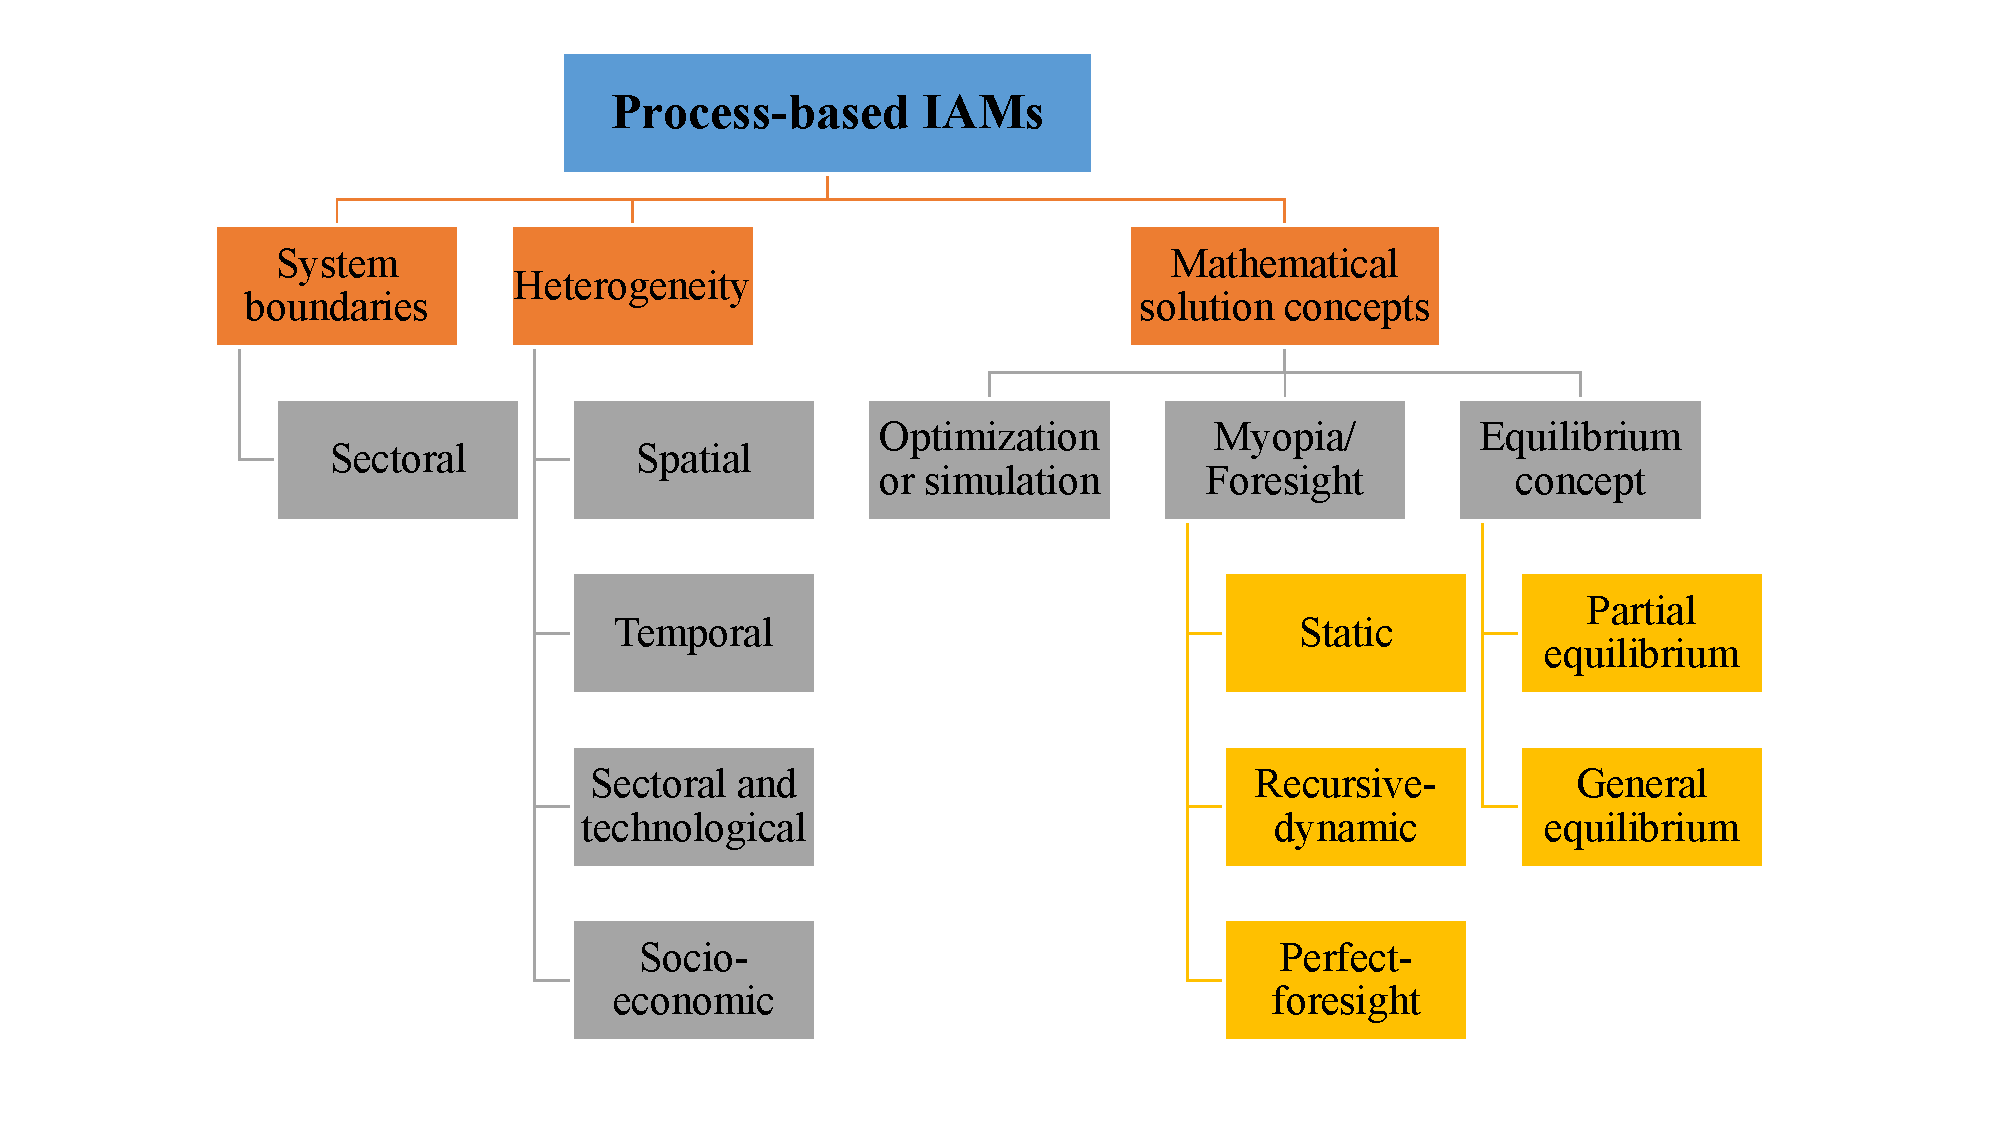
\includegraphics[width=\textwidth]{process_based_diff.pdf}
\caption{Diagram illustrating important points of difference between process-based IAMs. Own illustration based on classification by \citet{krey2014}.}
\label{fig:process_based}
\end{figure}

\subsection{Multimodel intercomparison studies}\label{subsec:model_inter}
Since models differ on a variety of aspects and integrate a complex suite of disciplines characterised by deep uncertainties, model evaluation becomes critical \citep{wilson2021,krey2014}. The aim of model evaluation is to assess the performance of the model in terms of how good they are for their intended use \citep{oreskes1998evaluation}. This in turn helps to improve their usefulness and robustness for policy analysis. One of the methods for model evaluation involves model inter-comparison projects (MIPs). These compare outputs and insights across a range of models by designing scenarios that harmonise key assumptions or drivers. These could be socio-economic developments \citep{riahi2017a}, policy assumptions \citep{tavoni2015post}, carbon budgets \citep{bertram2021}, technology assumptions \citep{bosetti2015sensitivity}, etc. The final aim is to generate robust insights that are to a large degree independent of modelling approaches and parametric assumptions \citep{krey2014}. 

\subsection{Global and National model intercomparison}\label{subsec:glonat}
Most of the studies mentioned in the preceding section consider only global models of integrated assessment. They include inter-regional trade, the pace and cost dynamics of new technologies, and the link between the global economy with the global climate system. Most of them are technology-rich, giving the energy system a variety of decarbonisation options. On the other hand, national models, which often only include the energy sector, generally consider national circumstances and constraints in more detail. A comparison of the two can thus lead to interesting insights in plausible country decarbonisation pathways.

\subsection{Committed emissions and stranded assets}\label{subsec:comm_stranded}

Energy infrastructure, particularly power plants, have long lifespans making them prone to path-dependence, thereby locking the system into a carbon-based trajectory \footnote{assuming infrastructure is based on fossil fuels.} and preventing alternatives to emerge. A number of studies have identified the risk of carbon lock-ins through near-term investment in fossil-fuel related infrastructure \citep[see e.g.,][]{bertramlockin2015,erickson2015,johnson2015}. Such lock-ins can occur for both developed nations, who plan to reduce their carbon intensity by investing in gas-based power, coal plants with higher efficiency, coal with CCS etc. and for developing nations, who wish to quickly expand power generation through build-up of (unabated) coal power. These can eventually bind nations to suboptimal power systems by preventing the entry of cheaper renewable energy and lead to stranding in the face of stringent mitigation policies. 

\begin{figure}[hbtp]
\centering
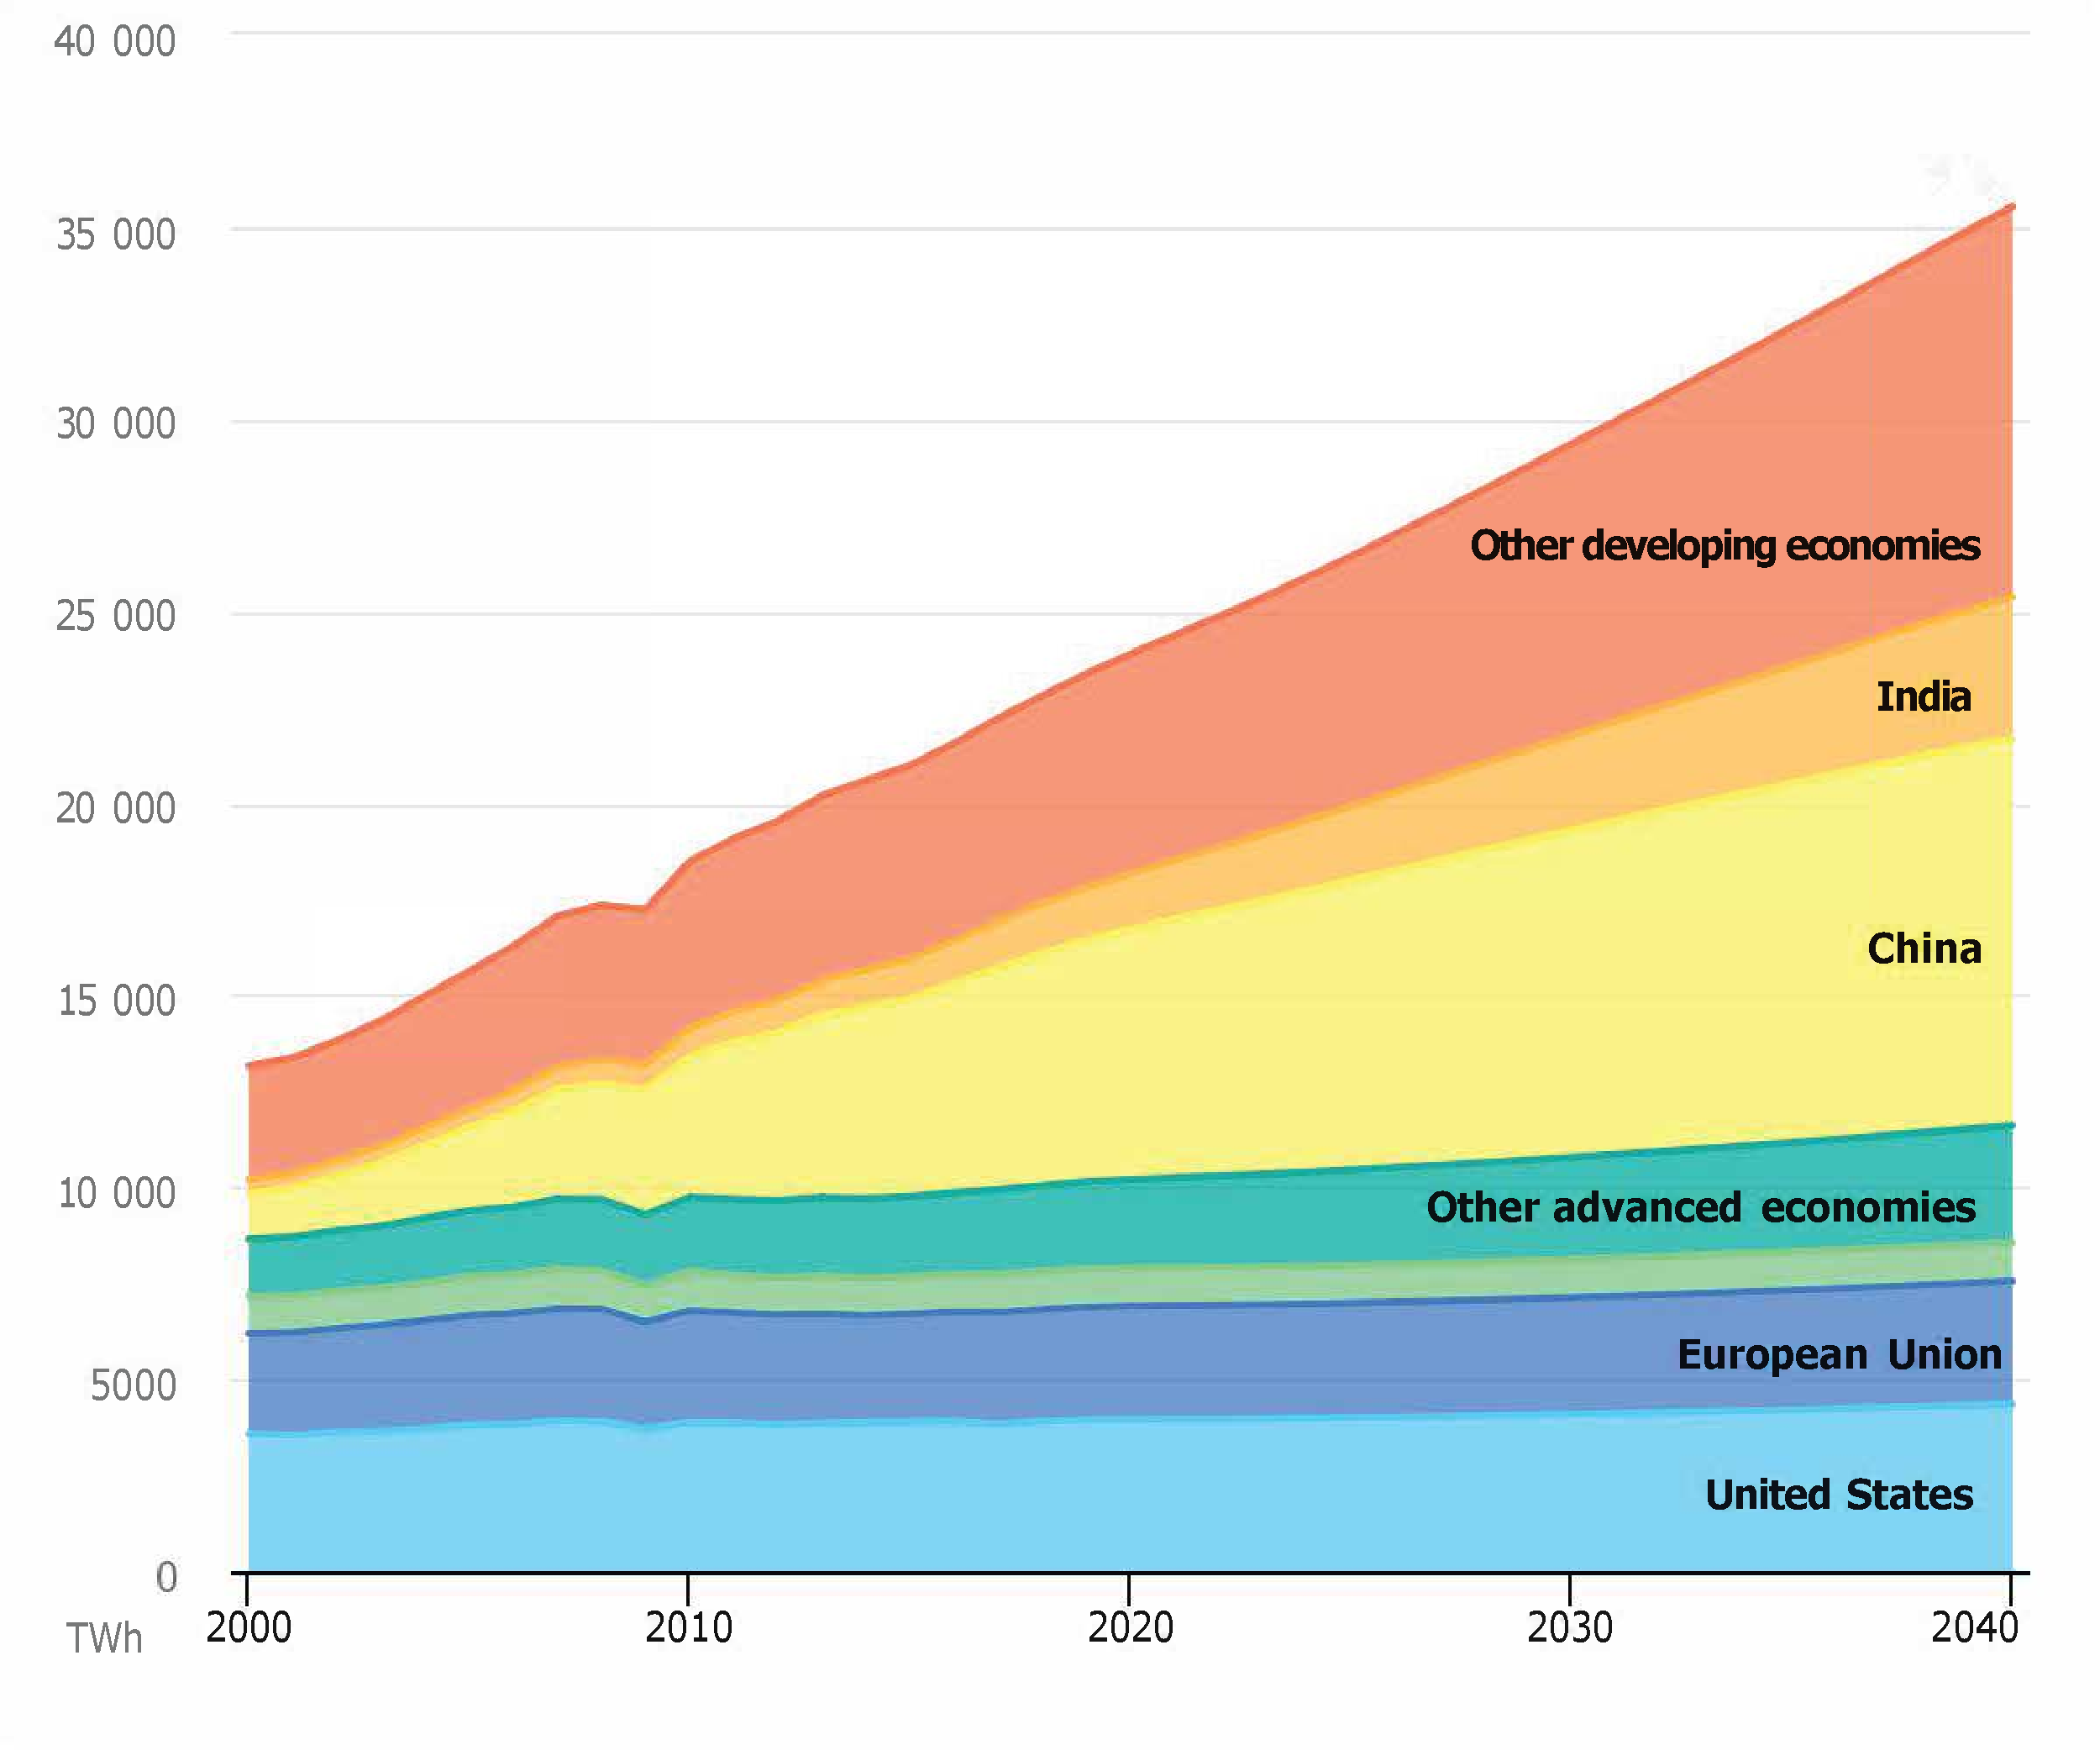
\includegraphics[width=\textwidth]{iea_demand_2.pdf}
\caption{Global electricity demand by region in the New Policies Scenario (IEA), 2000-2040 \citep{iea2019}}
\label{fig:iea_future}
\end{figure}

Two key interlinked metrics have been used to illustrate how this `infrastructure-inertia' \citep{davis2010future} affects mitigation, namely i) \textbf{committed emissions} and ii) \textbf{stranded assets}. Committed emissions refers to emissions resulting from continued (historical) use of CO2-emitting infrastructure. This infrastructure could either be already standing, under-construction, or planned. To convey the connection to mitigation action, \citet{tong2019committed} show that the committed fossil-fuel emissions from existing infrastructure  would alone exceed the \SI{1.5}{\degreeCelsius} carbon budget or consume two-thirds of the \SI{2}{\degreeCelsius} carbon budget. Moreover, over \SI{50}{\percent} of these emissions arise from power-plants. These shares climb even further when proposed power plants are taken into account. However, committed emissions is not a static concept: economy and policy-constraints greatly influence the lifetime and operation of energy infrastructure and from therein emerges the second metric of `stranded assets'. Defined broadly, a stranded asset refers to any piece of equipment that is used below its `expected operation and lifetime'. For a power plant, this is the unused capacity when a plant is operating below its designed load factor \citep{johnson2015}. This has the effect of reducing revenues for the generator and/or delaying the time when the generator accrues `enough' profits for the investment to be justified. In the worst case, the operating losses can force the plant to retire early. Stranded assets in the context of climate policy thus provide a measure of investment risk of existing and planned energy infrastructure as well as an indicator of resistance to be faced against stringent climate action.


\subsection{Employment assessment of energy policies} \label{sec:employment}

Methods of employment assessment can generally be divided into two main approaches, i) ex-post (bottom-up) analytic approach using employment factors, and ii) the use of (top-down) Input-Output (IO) or CGE models where employment is an internal modelled variable \citep{kammen2004,breitschopf2012}. The employment factor \footnote{In some studies also called as labour intensity \citep{simas2014,lambert2012}.} approach uses as labour market indicators the ratio of Full-time-equivalent jobs (FTE, sometimes called Jobs-year equivalent) to MW capacity (or MWh/year or dollars invested). These values are disaggregated into stages or activities of production (e.g., Manufacturing, Construction and Installation, etc.)\footnote{\citet{simas2014} even further disaggregate the activities, e.g., manufacturing into manufacture of components of a wind turbine - nacelle, rotor, blades, tower. }. These activities are then combined (depending on the activity) to actual and installed capacity, to get jobs by activity and sector (wind, solar). In comparison, IO and CGE models include the flow of goods and services between the  sectors of the economy; i.e., everything produced either serves as an input to the next level of production or has an end-use purpose \citep{irenaRenewableEnergyJobs2014}. This knowledge of inter-linkages between the economic sectors allows finding the macro-economic impacts (gross or net employment change), including employment, of various energy and climate policies  \citep{lambert2012}. 
Secondly, unlike the employment factor approach, where most studies restrict themselves to assessment of direct employment (in one sector), the I/O approach can often inform about indirect or induced effects (spanning other economic sectors). A summary of the two approaches including their advantages and limitations is shown in \Cref{table:empl_diff}.

\begin{figure}[h]
\centering
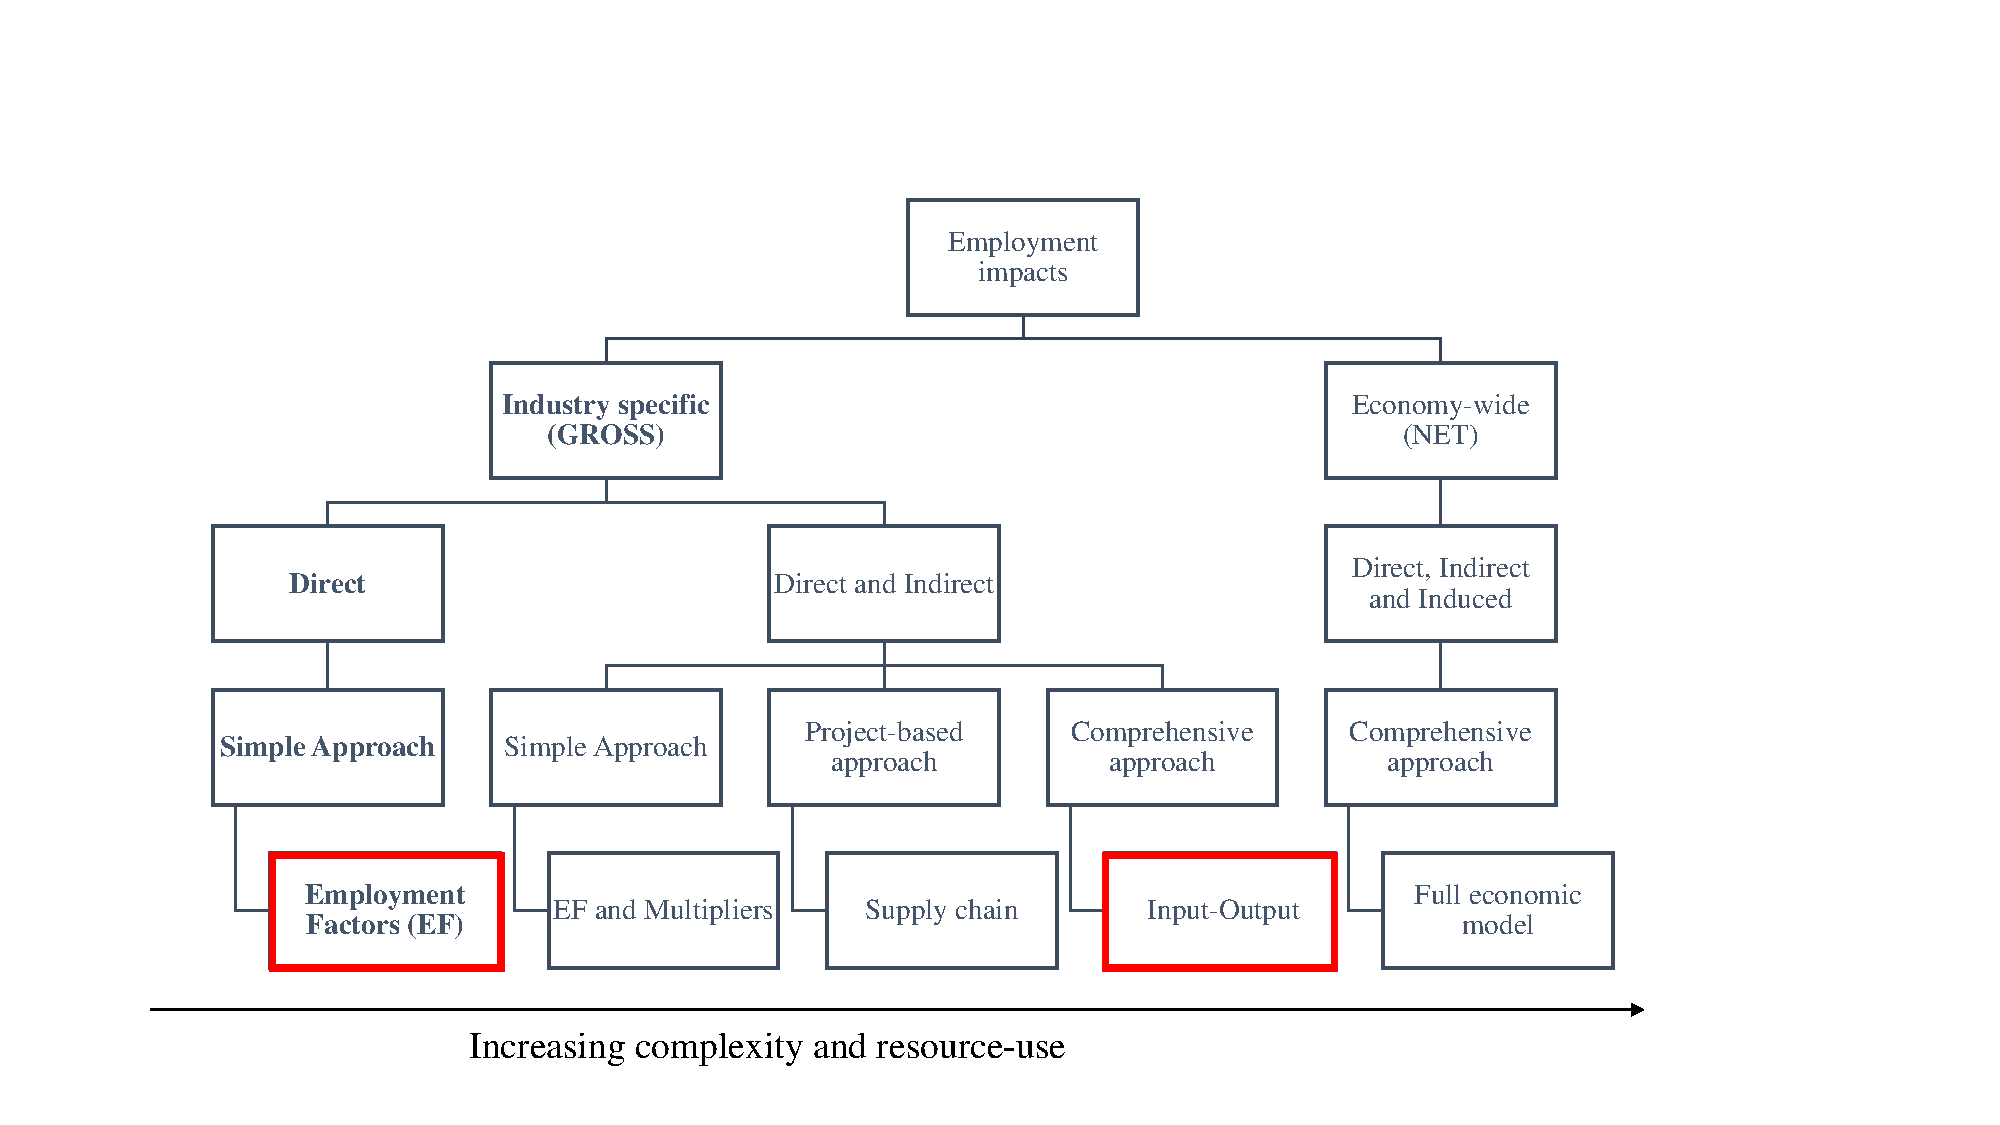
\includegraphics[width=\textwidth]{emp-structure.pdf}
\caption{Approaches to study employment impact; Elaborated by \citet{irenaRenewableEnergyJobs2014} based on \citet{breitschopf2012}.}
\label{fig:emp-structure}
\end{figure}

\begin{landscape}
\begin{table}[h]
       \begin{tabularx}{\textwidth}{|p{3cm}|p{3.5cm}|p{5cm}|X|}
    \hline
        Approach & Description & Advantages & Limitations \\ \hline
        Analytical - Employment factor approach & Generally combine employment factors produced from literature and industry surveys with energy sector data produced from an energy model or IAM & High level of transparency and simplicity \citep{cameron2015} & \begin{itemize} \item Reported employment factors for different technologies and activity can vary widely \citep{cameron2015} \item Cannot calculate indirect employment impacts \item Most studies of employment factors limited to OECD countries \item Few studies with employment factors of conventional technologies \end{itemize}    \\ \hline
        IO or CGE approaches &  & Allows for the consistent estimation of both direct and indirect effects due to inter-linkages between sectors & \begin{itemize} \item Imply a large burden in terms of data collection, as they require detailed knowledge of how industries are linked to one another \citep{cameron2015}\item Carries typical limitations of IO models: doesn't account for for time lags, homogeneity of outputs, high sectoral aggregation (doesn't resolve RE sectors), absence of economies of scale, invariance of technological coefficients and productivity, and missing interactions between prices and quantities     \citep{markandya2016,fragkos2018} \end{itemize}  \\ \hline
    \end{tabularx}
\caption{Table showing differences between the two broad types of approaches to measure employment impacts.}
\label{table:empl_diff}
\end{table}
\end{landscape}

The differences in methodological approaches, each with their advantages and limitations, and the scope of difference studies (direct, indirect, or induced employment) make comparison difficult. Even for studies using the same approach, there can a wide range of input values and key assumptions, making a one-to-one comparison difficult. 
 
\section{Structure of the thesis}
The three research questions introduced in \cref{sec:objectives} form the basis of the three core chapters of the thesis. The linking of the core chapters to the conceptual framework (\cref{sec:framework}) is illustrated in \Cref{fig:graphical_outline}. A solid one-way arrow shows a direct relation to the elements within the classifier whereas a dashed one-way arrow shows an indirect relation. Thus, Chapter \ref{ch:ERLPaper}: ``Reducing Stranded Assets through Early action in the Indian Power sector'' explores techno-economics barriers emerging from the risk of stranded assets. Chapter \ref{ch:EnPolPaper}: ``Climate Policy accelerates structural changes in energy employment'' investigates socio-economic and political barriers emerging from changes in energy employment, especially the loss of coal mining jobs. Chapter \ref{ch:ERLPaper2}: ``Early just transition opportunities for coal-bearing states of India'' again explores political barriers emerging from unequal distribution of energy assets in the country. Lastly, Chapter \ref{ch:summary} summarises the main findings of the three published studies, discusses their policy implications, identifies limitations, and suggests areas of future research work. The references to chapter \ref{ch:intro} and chapter \ref{ch:summary} are listed at the end of the thesis under `References', while references to chapters \ref{ch:ERLPaper}, \ref{ch:EnPolPaper}, and \ref{ch:ERLPaper2} are listed  after each chapter.

\begin{figure}[hbtp]
\centering
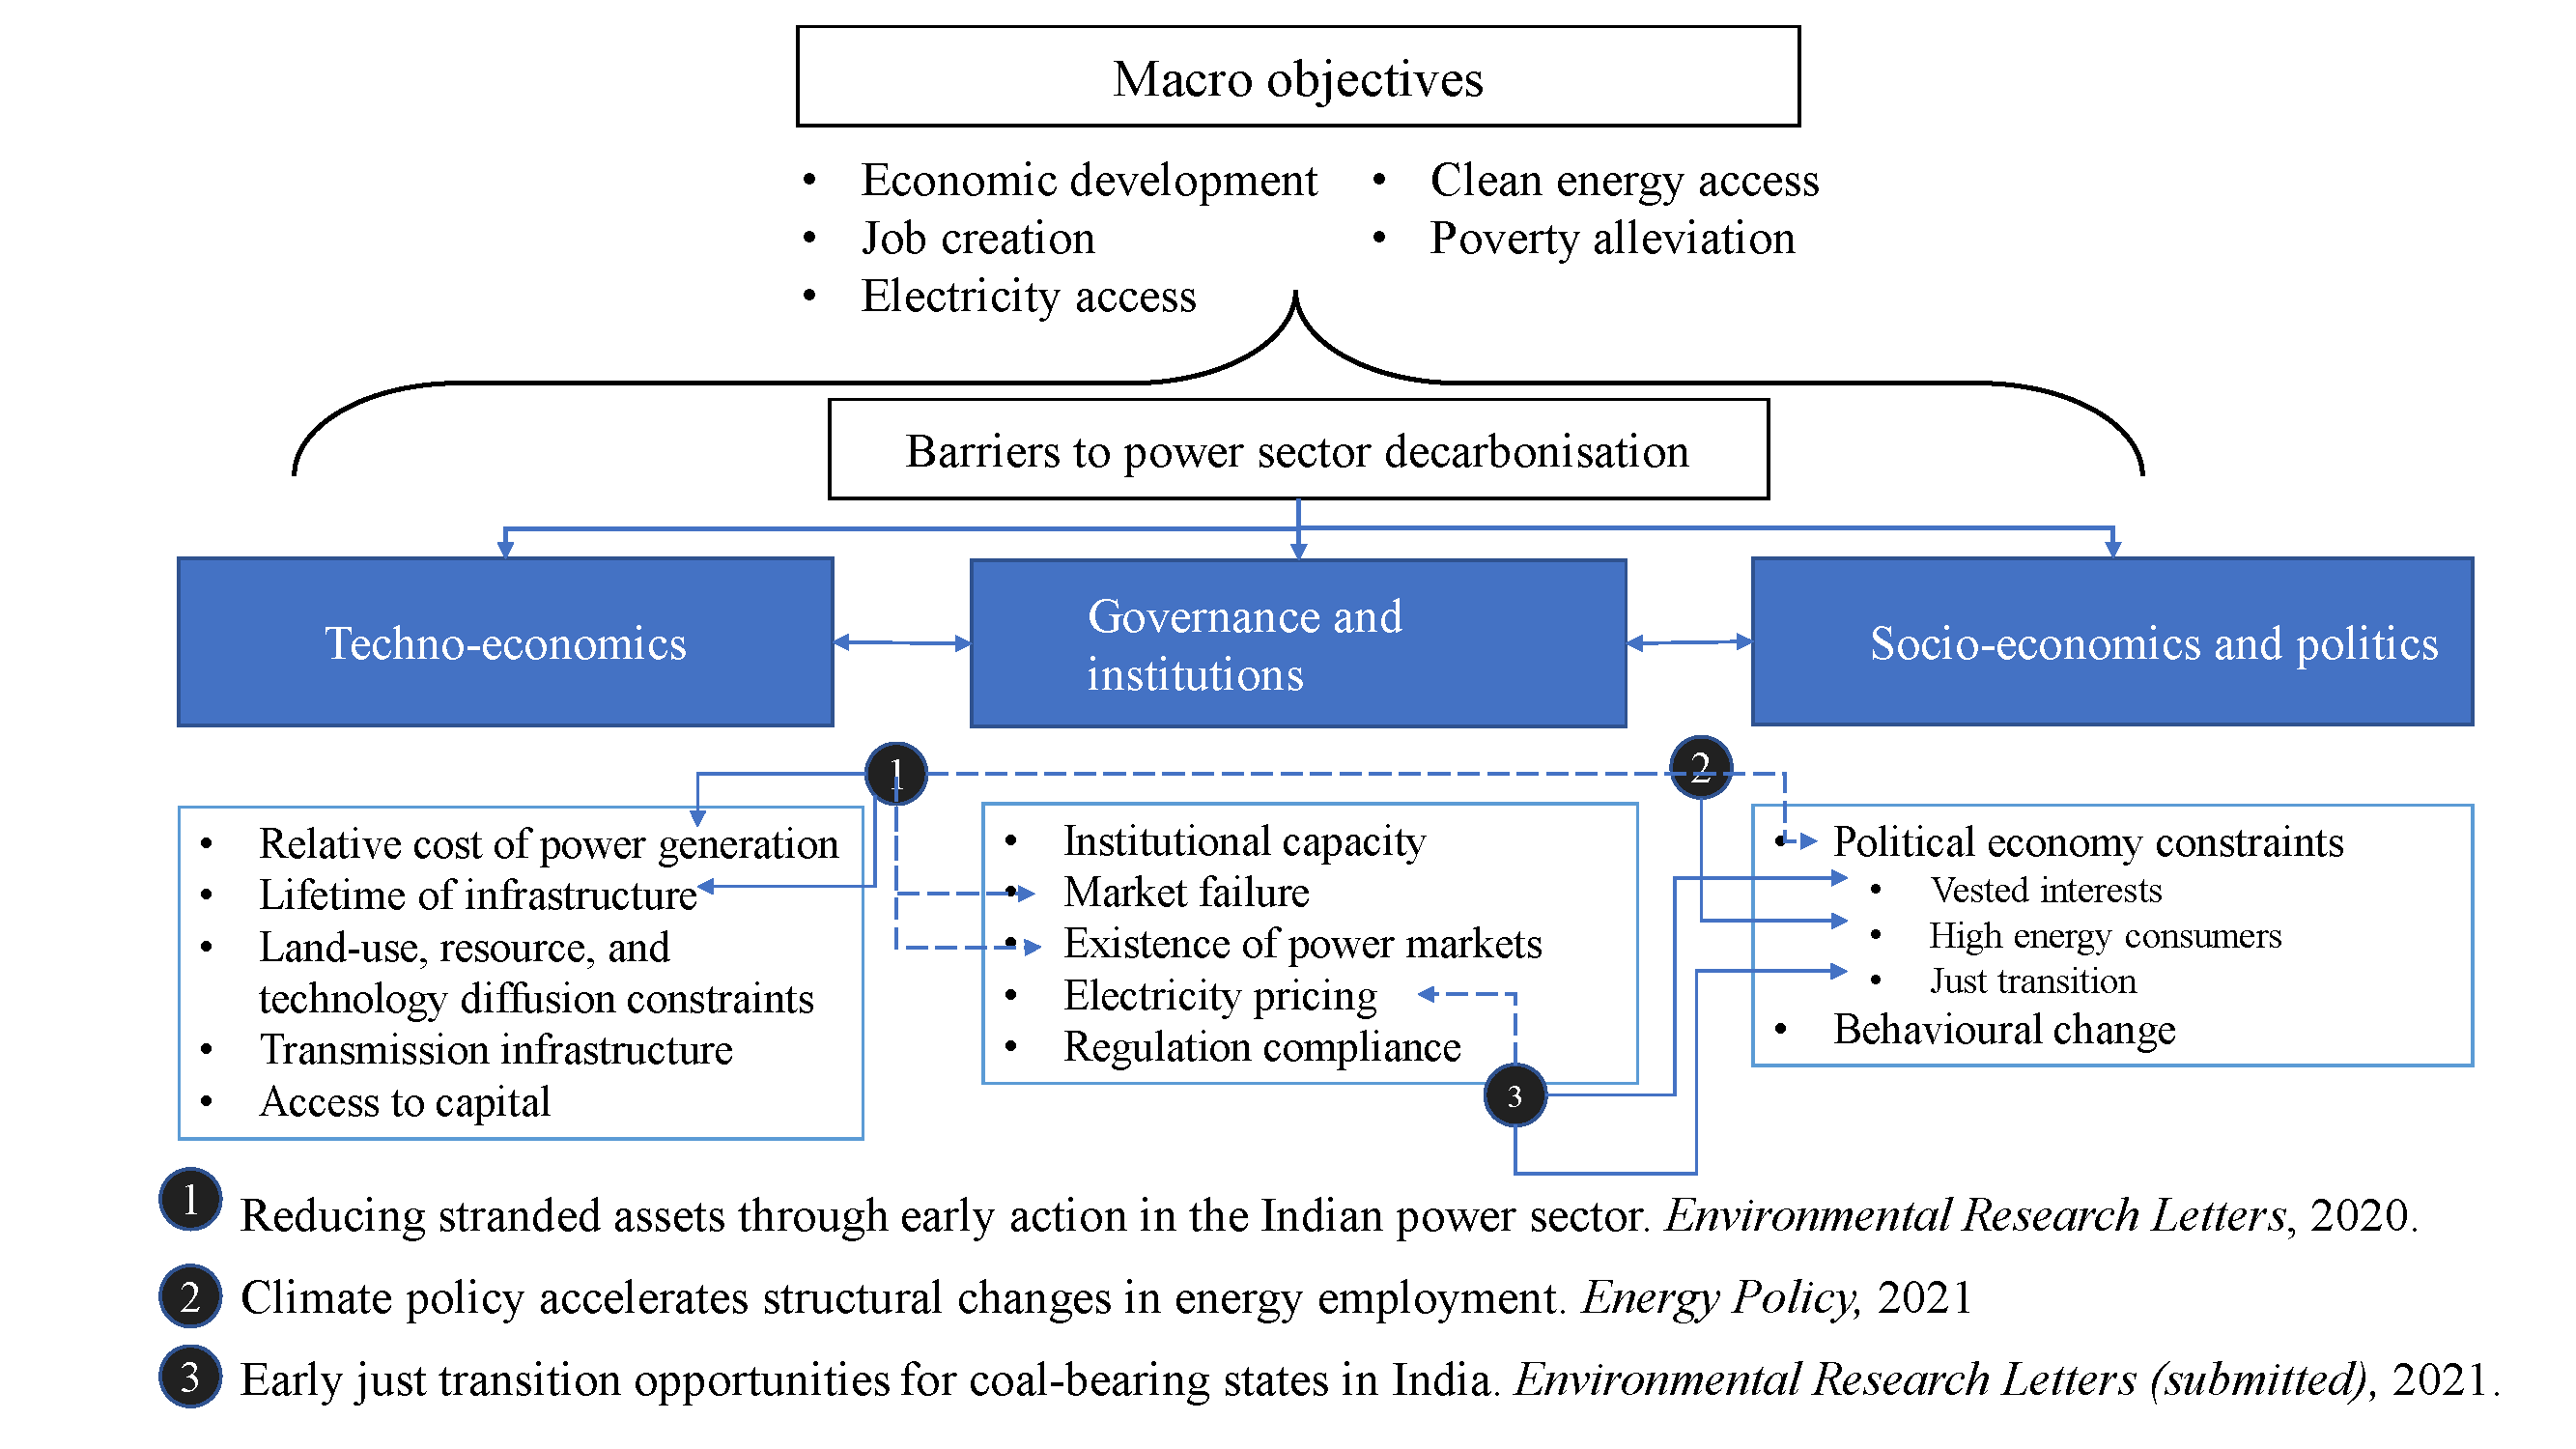
\includegraphics[width=\textwidth]{graphical_outline.png}
\caption{Objective and outline of the thesis, including where the different thesis chapters state in the conceptual framework. A solid one-way arrow shows a direct relation to the elements within the classifier whereas a dashed one-way arrow shows an indirect relation.}
\label{fig:graphical_outline}
\end{figure}


\biblio
\end{document}

